% !TEX root = ../McCoy-Dissertation.tex
\Appendix{Physics Introduction}\label{ap:x-ray_intro}
%%%%%%%%%%%%%%%%%%%%%e%%%%%%%%%%%%%%%%%%%%--------------------------------------------------
Basic physics relevant to this dissertation are outlined in \cref{ap:x-ray_intro,ap:quantum_spectral,app:x-ray_materials,ap:grating_basics} using SI units and the fundamental constants listed in \cref{tab:units,tab:fundamental_constants} throughout. 
\begin{table}[]
 \centering
 \caption[SI units for physical quantities]{Units for physical quantities in the \emph{System of International Units} (SI units) and SI derived units} \label{tab:units}
 \begin{tabular}{@{}llll@{}} 
 \toprule
 quantity & unit name & symbol & base units \\ \midrule 
 distance & meter & \si{\metre} & - \\
 time & second & \si{\second} & - \\
 mass & kilogram & \si{\kilogram} & - \\
 electric current & ampere & \si{\ampere} & - \\
 amount of substance & mole & \si{\mole}  & \num{6.02214076e23} \\ 
 temperature & kelvin & \si{\kelvin} & - \\ \midrule 
 energy & joule & \si{\joule} & \si{\kilogram\square\metre\per\square\second} \\
 power & watt & \si{\watt} & \si{\kilogram\square\metre\per\second\tothe{3}} \\ 
 electric charge & coulomb & \si{\coulomb} & \si{\ampere\second} \\
 electric potential & volt & \si{\volt} & \si{\kilogram\square\metre\per\ampere\per\second\tothe{3}} \\
 electrical resistance & ohm & \si{\ohm} & \si{\kilogram\square\metre\per\ampere\tothe{2}\per\second\tothe{3}} \\
 electrical capacitance & farad & \si{\farad} & \si{\second\tothe{4}\ampere\tothe{2}\per\square\metre\per\kilogram} \\
 electrical inductance & henry & \si{\henry} & \si{\kilogram\square\metre\per\square\second\per\square\ampere} \\
 magnetic flux density & tesla & \si{\tesla} & \si{\kilogram\per\square\second\per\ampere} \\
 pressure & pascal & \si{\pascal} & \si{\kilogram\per\metre\per\square\second} \\ %\\
 %temperature & degree Celsius & \si{\celsius} & $\SI{0}{\celsius} = \SI{273.15}{\kelvin}$ \\ 
 \bottomrule
 \end{tabular}
 \end{table}
\begin{table}[]
 \centering
 \caption[Relevant physical constants in SI units]{Physical constants expressed in SI units and definition of the electronvolt (the amount of energy that an electron posses after passing through an electric potential difference of one volt).} \label{tab:fundamental_constants}
 \begin{tabular}{@{}lll@{}} 
 \toprule
 quantity & symbol & value in SI units \\ \midrule 
 \emph{Planck's constant} & $h$ & \SI{6.62607015e-34}{\joule\second} \\ 
 \emph{reduced Planck's constant} & $\hbar \equiv h / 2 \pi$ & \SI{1.05457800e-34}{\joule\second} \\ 
 \emph{vacuum permittivity} & $\epsilon_0$ & \SI{8.85418782e-12}{\farad\per\metre} \\ 
 \emph{vacuum permeability} & $\mu_0$ & \SI{4 \numpi e-7}{\henry\per\metre} \\ 
 \emph{speed of light (in vacuum)} & $c_0 \equiv \left( \epsilon_0 \mu_0 \right)^{-1/2}$ & \SI{299792458}{\metre\per\second} \\ 
 \emph{impedance of free space} & $Z_0 \equiv \mu_0 c_0$ & \SI{119.9169832 \numpi}{\ohm} \\
 \emph{elementary charge} & $q_e$ & \SI{1.60217662e-19}{\coulomb} \\ 
 \emph{electron rest mass} & $m_e$ & \SI{9.1093835e-31}{\kilogram} \\ 
 \emph{Bohr radius} & $a_0 \equiv 4 \pi \epsilon_0 \hbar^2 / m_e q_e^2$ & \SI{5.2917721067e-11}{\metre} \\ 
 \emph{classical electron radius} & $r_e \equiv q_e^2 / 4 \pi \epsilon_0 m_e c_0^2$ & \SI{2.81794032e-15}{\metre} \\
 \emph{Rydberg constant} & $R_{\infty} \equiv m_e q_e^4 / 8 \epsilon_0^2 h^3 c_0$ & \SI{10973731.568508}{\per\metre} \\ 
 \emph{Thomson cross-section} & $\sigma_e \equiv 8 \pi r_e^2 / 3$ & \SI{6.6524587e-29}{\metre\square} \\
 \emph{Boltzmann constant} & $k_{\mathcal{B}}$ & \SI{1.380648e-23}{\joule\per\kelvin} \\
 \emph{fine-structure constant} & $\alpha_f \equiv q^2_e / 4 \pi \epsilon_0 \hbar c_0$ & \num{0.0072973525693} $\approx 1/137$ \\ \midrule
 \emph{electronvolt} & \SI{1}{\electronvolt} & \SI{1.6021766209e-19}{\joule} \\ 
 %\emph{centigrade} & \si{\celsius} & $\SI{0}{\celsius} = \SI{273.15}{\kelvin}$ \\
 \bottomrule
 \end{tabular}
 \end{table}
To start, all types of electromagnetic radiation can be described physically as both classical electromagnetic waves and massless particles (\emph{i.e.}, \emph{photons}) according to \emph{wave-particle duality}. 
This principle was first proposed by Planck and Einstein in the early 1900s \cite{Planck1901,Einstein1905a} and later validated by Compton in the early 1920s through the discovery of \emph{Compton scattering}, where x-rays transfer momentum to electrons as they are ejected from atoms \cite{Compton23a,Als-Nielsen11}. 
While this process can usually be neglected for radiation with wavelength, $\lambda$, much longer than the \emph{Compton wavelength} of the electron ($\lambda_C \equiv h / m_e c_0 \approx$~\SI{2.43}{\pico\metre}) [\emph{cf.\@} \cref{eq:electron_wavelength}], their interaction with matter can still be explained in terms of particle-like excitations in the quantized electromagnetic field with photon energy, $\hbar \omega$, and momentum, $\hbar \mathbold{k}$ \cite{Townsend00,Shankar04}. 
Equivalently, electromagnetic radiation can be understood from a classical perspective to be coupled oscillations in the \emph{electric field}, $\mathbold{E}(\mathbold{r},t)$, and \emph{the magnetic field}, $\mathbold{B}(\mathbold{r},t)$, that propagate together at the speed of light, $c_0$ \cite{Jackson75,Born80}. 
Across the electromagnetic spectrum, radiation tends to interact with matter on size scales comparable to its wavelength [\emph{cf.\@} \cref{tab:EM_spectrum}]. 
\begin{table}[]
 \centering
 \caption{Approximate wavelength ranges for all types of electromagnetic radiation}\label{tab:EM_spectrum}
 \begin{tabular}{@{}lll@{}} 
 \toprule
 spectral band & wavelength range & comparison \\ \midrule 
 radio waves & $\gtrapprox$ \SI{1}{\metre} & large objects \\ 
 microwaves & \SI{1}{\metre} to \SI{1}{\milli\metre} & meter stick \\ 
 terahertz radiation & \SI{1}{\milli\metre} to \SI{100}{\micro\metre} & grain of salt \\ 
 infrared radiation & \SI{100}{\micro\metre} to \SI{700}{\nano\metre} & human hair thickness, biological cells \\ 
 visible light & \SI{700}{\nano\metre} to \SI{400}{\nano\metre} & bacteria \\ 
 ultraviolet radiation & \SI{400}{\nano\metre} to \SI{5}{\nano\metre} & viruses, large molecules \\ 
 x-rays & \SI{5}{\nano\metre} to \SI{1}{\pico\metre} & atoms \\
 gamma rays &  $\lessapprox$ \SI{1}{\pico\metre} & atomic nuclei \\ 
 \bottomrule
 \end{tabular}
 \end{table}
Falling at the red end of the x-ray spectrum, soft x-rays have $\lambda$ approaching the atomic scale with high frequency $\omega = 2 \pi c_0 / \lambda$ comparable to atomic resonances in relatively light elements \cite{Attwood17}. 
To provide physics background for \cref{ch:introduction,ch:diff_eff,ap:quantum_spectral,app:x-ray_materials,ap:grating_basics}, this appendix outlines basics of classical-wave and photon descriptions for soft x-rays and their interaction with atomic electrons under the framework of non-relativistic quantum mechanics. 

\section{X-ray Nomenclature}\label{sec:histroical}
%%%%%%%%%%%%%%%%%%%%%%%%%%%%%%%%%%%%%%%%%-------------------------------------------------
The defining feature of x-rays that led to their discovery is their ability to penetrate through certain materials.
In R\"ontgen's experiments of the 1890s \cite{Rontgen1898a,Rontgen1898b,Rontgen1896}, x-rays were mainly produced by the deceleration of electrons as \emph{bremmstrahlung}, or ``braking radiation'' in an early electric discharge tube \cite{Compton35,Rybicki86,Attwood17,Als-Nielsen11}.\footnote{X-ray spectral lines characteristic of fluorescence occurring in the anode are also produced.} 
Such a device consists of a glass bulb that houses two electrodes held under partial vacuum while an applied high voltage (the \emph{tube voltage}, $V_T$) produces electric discharge from the negatively-biased cathode \cite{Coolidge1913,Compton35,Als-Nielsen11}. 
When tube voltages on the order of tens of \si{\kilo\volt} up to \SI{100}{\kilo\volt} were applied to the apparatus, it was found that a \emph{new kind of ray}, or \emph{x-ray}, with a unique penetrating ability was produced \cite{Rontgen1898a,Rontgen1896}. 
This then-unknown form of radiation was detected through observing fluorescence in barium platinocyanide (Ba[Pt(CN)$_4$]), which was coated on a screen nearby the electric discharge tube, where it was discovered that even with the apparatus covered in light-blocking cardboard and the room darkened, Ba[Pt(CN)$_4$] produced a fluorescent glow when tube voltages up to \SI{100}{\kilo\volt} were applied. 

R\"ontgen discovered that radiation produced by $V_T \lessapprox \SI{100}{\kilo\volt}$ was able to penetrate though relatively low-$\mathcal{Z}$ materials such as cardboard whereas it was easily absorbed by heavier materials, such as pieces of metal lab equipment. %\footnote{On this note, R\"ontgen discovered that human bone, being rich in calcium ($\mathcal{Z}=20$), tends to absorb hard x-rays significantly more than the surrounding soft tissue. This enabled the first x-ray photograph of a human body part, which effectively gave birth to the radiographic techniques used in fields such as medicine and dentistry today \cite{Mould1995}.}   
With the maximum photon energy generated by bremmstrahlung being $q_e V_T$, x-rays with $\hbar \omega$ ranging from tens of \si{\kilo\electronvolt} to \SI{100}{\kilo\electronvolt} are referred to as \emph{hard x-rays} for this historical reason \cite{Als-Nielsen11}. 
On the other hand, radiation produced by $V_T \sim \SI{1}{\kilo\volt}$ was observed to be easily absorbed by virtually any material in early experiments, and as a result, x-rays with $ \SI{200}{\electronvolt}\lessapprox \hbar \omega \lessapprox \SI{2}{\kilo\electronvolt}$ are referred to as \emph{soft x-rays} \cite{Attwood17}. %[\emph{cf.\@} \cref{sec:SXR_med}]
However, these definitions vary in the literature and additionally, intermediate x-rays with $\SI{1}{\kilo\electronvolt} \lessapprox \hbar \omega \lessapprox \SI{5}{\kilo\electronvolt}$ are sometimes called \emph{tender x-rays} \cite{Northrup16,Senf16}.

\section{Photons and Classical Electromagnetic Waves}\label{sec:EM_waves_vac}
%%%%%%%%%%%%%%%%%%%%%%%%%%%%%%%%%%%%%%%%%--------------------------------------------------
The behavior of electromagnetic waves is governed by \emph{Maxwell's equations}, which are the foundation for classical electrodynamics \cite{Landau60,Jackson75,Born80,Rybicki86,Kahn02,Griffiths17,Attwood17}. 
In their microscopic form, these four equations are:\footnote{Throughout this thesis, $\cdot$ indicates a scalar (\emph{dot}) product while $\times$ indicates a vector (\emph{cross}) product such that $\divergence$ and $\curl$ represent \emph{divergence} and \emph{curl} vector operators, respectively.} 
\begin{subequations}
\begin{align}
 \div \mathbold{E}(\mathbold{r},t) &= \frac{\rho(\mathbold{r},t)}{\epsilon_0} \label{eq:Maxwell_vac_start_1} \\
 \curl \mathbold{E}(\mathbold{r},t) &= - \pdv{\mathbold{B}(\mathbold{r},t)}{t} \label{eq:Maxwell_vac_start_2}\\
 \div \mathbold{B}(\mathbold{r},t) &= 0 \label{eq:Maxwell_vac_start_3} \\
 \curl \mathbold{B}(\mathbold{r},t) &= \mu_0 \mathbfcal{J}(\mathbold{r},t) + \frac{1}{c_0^2} \pdv{\mathbold{E}(\mathbold{r},t)}{t}, \label{eq:Maxwell_vac_start_4}
 \end{align}
\end{subequations}
where $\epsilon_0$ is the vacuum permittivity and $\mu_0$ is the vacuum permeability with the speed of light given by $c_0 \equiv \left( \epsilon_0 \mu_0 \right)^{-1/2}$ [\emph{cf.\@} \cref{tab:fundamental_constants}]. 
Additionally, $\rho(\mathbold{r},t)$ is the volume density of electric charge and $\mathbfcal{J}(\mathbold{r},t)$ is a directional electric current density; these quantities are related to each other through the following \emph{continuity equation}:
\begin{equation} \label{eq:continuity}
 \divergence \mathbfcal{J}(\mathbold{r},t) + \pdv{\rho(\mathbold{r},t)}{t} = 0 , 
 \end{equation}
which ensures that electric charge is conserved \cite{Landau60,Jackson75,Born80,Rybicki86,Griffiths17,Attwood17}. 
The basic laws of electromagnetism are described by \cref{eq:Maxwell_vac_start_1,eq:Maxwell_vac_start_2,eq:Maxwell_vac_start_3,eq:Maxwell_vac_start_4}: 
\begin{enumerate}[noitemsep]
	\item \cref{eq:Maxwell_vac_start_1} is \emph{Gauss's law}, which describes how electric field lines diverge from a source of electric charge $\rho(\mathbold{r},t)$ (\emph{i.e.}, $\div \mathbold{E}(\mathbold{r},t) \neq 0$) %\cite{Lagrange1869,Gauss1877}
	\item \cref{eq:Maxwell_vac_start_2} is \emph{Faraday's law of induction}, which states that a dynamic magnetic field (\emph{i.e.}, $\pdv{\mathbold{B}(\mathbold{r},t)}{t} \neq 0$) generates a curled electric field (\emph{i.e.}, $\curl \mathbold{E}(\mathbold{r},t) \neq 0$)
	\item \cref{eq:Maxwell_vac_start_3} is a statement that magnetic charge does not exist and hence magnetic field lines are never divergent (\emph{i.e.}, $\div \mathbold{B}(\mathbold{r},t) = 0$ always)
	\item \cref{eq:Maxwell_vac_start_4} is the \emph{Amp\`ere-Maxwell equation}, an extension of \emph{Amp\`ere's circuital law}, which describes how an electric current with a density $\mathbfcal{J}(\mathbold{r},t)$ generates a curled magnetic field (\emph{i.e.}, $\curl \mathbold{B}(\mathbold{r},t) \neq 0$); Maxwell's correctional term, $\left( 1 / c_0^2 \right) \pdv*{\mathbold{E}(\mathbold{r},t)}{t}$, states that a a dynamic electric field also generates a curled magnetic field
\end{enumerate}

In vacuum, electric charge and electric current are null but it can be shown that wave behavior arises from Maxwell's equations provided that there is some far-away source that generates a dynamic electric or magnetic field. 
Maxwell's equations given by \cref{eq:Maxwell_vac_start_1,eq:Maxwell_vac_start_2,eq:Maxwell_vac_start_3,eq:Maxwell_vac_start_4} for this situation read as
\begin{subequations}
\begin{align}
 \div \mathbold{E}(\mathbold{r},t) &= 0 \label{eq:Maxwell_vac_1}  \\
 \curl \mathbold{E}(\mathbold{r},t) &= - \mu_0 \pdv{\mathbold{H}(\mathbold{r},t)}{t}  \label{eq:Maxwell_vac_2} \\
 \div \mathbold{H}(\mathbold{r},t) &= 0 \label{eq:Maxwell_vac_3}  \\
 \curl \mathbold{H}(\mathbold{r},t) &= \epsilon_0 \pdv{\mathbold{E}(\mathbold{r},t)}{t} . \label{eq:Maxwell_vac_4}
 \end{align}
\end{subequations}
For convenience of notation, the \emph{auxiliary magnetic field}, $\mathbold{H}(\mathbold{r},t)$, has been substituted for the \emph{fundamental magnetic field}, $\mathbold{B}(\mathbold{r},t)$, through the constitutive relation $\mathbold{B}(\mathbold{r},t) = \mu_0 \mathbold{H}(\mathbold{r},t)$ \cite{Landau60,Jackson75,Griffiths17}.\footnote{This constitutive relation holds in vacuum and also in non-magnetized media, which need not be discussed in this context. Because of this, $\mathbold{B}(\mathbold{r},t)$ and $\mathbold{H}(\mathbold{r},t)$ are both referred to as \emph{the magnetic field} in this thesis.} 
Qualitatively, \cref{eq:Maxwell_vac_1,eq:Maxwell_vac_3} state that field lines are non-divergent while \cref{eq:Maxwell_vac_2,eq:Maxwell_vac_4} describe how a time-varying $\mathbold{H}(\mathbold{r},t)$ leads to a curled $\mathbold{E}(\mathbold{r},t)$ and vice-versa. 
These conditions can be seen to lead to wave behavior by combining \cref{eq:Maxwell_vac_1,eq:Maxwell_vac_2,eq:Maxwell_vac_3,eq:Maxwell_vac_4}\footnote{In particular, this can be done by first taking curls of \cref{eq:Maxwell_vac_2,eq:Maxwell_vac_4}: 
\begin{align*}
 \begin{split}
 \curl \curl \mathbold{E}(\mathbold{r},t) &= \grad \left[\div \mathbold{E}(\mathbold{r},t)\right] - \laplacian \mathbold{E}(\mathbold{r},t) = - \mu_0 \pdv{\left[ \curl \mathbold{H} (\mathbold{r},t) \right]}{t} = - \epsilon_0 \mu_0 \pdv[2]{\mathbold{E}(\mathbold{r},t)}{t}\\
 \curl \curl \mathbold{H}(\mathbold{r},t) &= \grad \left[\divergence \mathbold{H}(\mathbold{r},t)\right] - \laplacian \mathbold{H}(\mathbold{r},t) = \epsilon_0 \pdv{\left[ \curl \mathbold{E} (\mathbold{r},t) \right]}{t} = - \epsilon_0 \mu_0 \pdv[2]{\mathbold{H}(\mathbold{r},t)}{t}
 \end{split}
 \end{align*}
and then inserting \cref{eq:Maxwell_vac_1,eq:Maxwell_vac_3}. 
 \label{footnote:combine}} to arrive at the following identical expressions for $\mathbold{E}(\mathbold{r},t)$ and $\mathbold{H}(\mathbold{r},t)$:
\begin{equation} \label{eq:wave_vector_vac}
 \left( \laplacian - \epsilon_0 \mu_0 \pdv[2]{t} \right) \left\{
  \begin{array}{lr}
  \mathbold{E}(\mathbold{r},t)\\
  \mathbold{H}(\mathbold{r},t)
  \end{array}
 \right\} = \mathbf{0} ,
 \end{equation}
where $\mathbf{0}$ is the null vector. 
Considering each component of $\mathbold{E}(\mathbold{r},t)$ and $\mathbold{H}(\mathbold{r},t)$ separately, this is equivalent to six scalar differential equations that each take the form of the scalar \emph{wave equation} \cite{Born80,Griffiths17}: 
\begin{equation} \label{eq:scalar_wave_general}
 \left( \laplacian + \frac{1}{v_p^2} \pdv[2]{t} \right) u (\mathbold{r},t) = 0 ,
 \end{equation}
where the scalar field $u (\mathbold{r},t)$ represents the wave medium and $v_p = c_0 \equiv \left( \epsilon_0 \mu_0 \right)^{-1/2}$ is the wave propagation speed. 
While other types of waves are described by this scalar wave equation (\emph{e.g.}, water waves, sound waves, etc.), classical electromagnetic waves are oscillations in the vector fields $\mathbold{E}(\mathbold{r},t)$ and $\mathbold{H}(\mathbold{r},t)$ and thus a full vector treatment is generally required to describe their behavior.\footnote{However, in situations where it can be assumed that $\mathbold{E}(\mathbold{r},t)$ continuously oscillates along the same axis (\emph{i.e.}, if the light is \emph{linearly polarized} to a high degree), only one scalar component need be considered. 
Then, \cref{eq:scalar_wave_general} with $v_p = c_0$ can be used to evaluate wave behavior while the other components of $\mathbold{E}(\mathbold{r},t)$ and $\mathbold{H}(\mathbold{r},t)$ follow from \cref{eq:Maxwell_vac_1,eq:Maxwell_vac_2,eq:Maxwell_vac_3,eq:Maxwell_vac_4}. See also \cref{ap:grating_basics}.}

\subsection{Time-Harmonic Classical Wave Modes}\label{sec:time_harmonic}
%%%%%%%%%%%%%%%%%%%%%%%%%%%%%%%%%%%%%%%%%--------------------------------------------------
Oscillatory solutions to \cref{eq:scalar_wave_general} are commonly discussed as normal modes with some singular value for $\omega$ such that if the scalar field $u (\mathbold{r},t)$ were continuously measured at a fixed position $\mathbold{r}_0$, a sinusoidal function would be generated: 
\begin{subequations}
\begin{equation}\label{eq:cosine_mode}
 u (\mathbold{r}_0,t) \equiv u (t) = u_0 \cos \left( \Phi - \omega t \right) ,
 \end{equation}
where $u_0$ is the amplitude of the wave and $\Phi$ is its phase. 
Alternatively, this can be expressed as a complex phasor: 
\begin{equation}\label{eq:phasor_mode}
 u (t) = u_0 \mathrm{e}^{i \left( \Phi - \omega t \right)} ,
 \end{equation} 
\end{subequations}
with $i \equiv \sqrt{-1}$ as the imaginary unit. 
However, realistic electromagnetic waves tend to exist in superpositions of these normal modes such that there is always some spread in $\omega$ \cite{Born80}. 
This can be gleaned from the temporal Fourier transforms of the electromagnetic fields:
\begin{equation}\label{eq:temporal_fourier}
 \left\{
 \begin{array}{lr}
 \mathbold{E} \left( \mathbold{r} , \omega \right) \\
 \mathbold{H} \left( \mathbold{r} , \omega \right)
 \end{array}
 \right\} = \int_{-\infty}^{\infty} \left\{
 \begin{array}{lr}
 \mathbold{E} \left( \mathbold{r} , t ' \right) \\
 \mathbold{H} \left( \mathbold{r} , t ' \right)
 \end{array}
 \right\} \mathrm{e}^{i \omega  t'} \dd{t'} ,
 \end{equation}  
where $\mathbold{E} \left( \mathbold{r} , \omega \right)$ and $\mathbold{H} \left( \mathbold{r} , \omega \right)$ can have singular values only if $\mathbold{E} \left( \mathbold{r} , t \right)$ and $\mathbold{H} \left( \mathbold{r} , t \right)$ are pure sinusoids lasting for a formally infinite amount of time. 
Conversely, the most general solution to \cref{eq:wave_vector_vac} is a superposition of normal wave modes spanning all values of $\omega$, which can be represented using the following inverse Fourier transforms of the electromagnetic fields:
\begin{equation}
 \left\{
 \begin{array}{lr}
 \mathbold{E} \left( \mathbold{r} , t \right) \\
 \mathbold{H} \left( \mathbold{r} , t \right)
 \end{array}
 \right\} = \frac{1}{2 \pi} \int_{-\infty}^{\infty} \left\{
 \begin{array}{lr}
 \mathbold{E} \left( \mathbold{r} , \omega ' \right) \\
 \mathbold{H} \left( \mathbold{r} , \omega ' \right)
 \end{array}
 \right\} \mathrm{e}^{-i \omega ' t} \dd{\omega} ' . 
 \end{equation} 
For simplicity, however, it is useful to imagine a wave that extends infinitely in time and space so that just one frequency mode is present.\footnote{This can be written by making the following replacement:
\begin{equation*}
 \left\{
 \begin{array}{lr}
 \mathbold{E} \left( \mathbold{r} , \omega ' \right) \\
 \mathbold{H} \left( \mathbold{r} , \omega ' \right)
 \end{array} 
 \right\} \to \left\{
 \begin{array}{lr}
 \mathbold{E} \left( \mathbold{r} \right) \\
 \mathbold{H} \left( \mathbold{r} \right)
 \end{array} 
 \right\} \delta_D \left( \omega ' - \omega \right) 
 \end{equation*} 
with $\delta_D (\omega ' - \omega)$ being a \emph{Dirac delta function}, which is defined as \begin{equation*}
\delta_D \left( x \right) \equiv
   \begin{cases}
     \infty, & \text{if}\ x = 0 \\
     0, & \text{if}\ x \neq 0 .
   \end{cases} 
\end{equation*}
\label{footnote:dirac_delta}}  %with $\ell_{\text{coh}} \to \infty$
In this case, the electromagnetic fields can be written as 
\begin{equation}\label{eq:single-mode}
 \left\{
 \begin{array}{lr}
 \mathbold{E} \left( \mathbold{r} , t \right) \\
 \mathbold{H} \left( \mathbold{r} , t \right)
 \end{array} 
 \right\} =  \left\{
 \begin{array}{lr}
 \mathbold{E} \left( \mathbold{r} \right) \\
 \mathbold{H} \left( \mathbold{r} \right)
 \end{array} 
 \right\} \mathrm{e}^{-i \omega t} , 
 \end{equation} 
where $\mathbold{E}(\mathbold{r})$ and $\mathbold{H}(\mathbold{r})$ are the \emph{time-harmonic} fields, which implicitly assume a $\mathrm{e}^{-i \omega t}$ time dependence. 

Electromagnetic fields oscillating in time necessarily have a corresponding spatial frequency. 
In other words, a normal mode of frequency $\omega$ at a fixed time time $t_0$ exhibits periodicity as a function of $\mathbold{r}$; essentially, this is the wavelength of the radiation.  
This can be deduced by inserting \cref{eq:single-mode} into \cref{eq:Maxwell_vac_1,eq:Maxwell_vac_2,eq:Maxwell_vac_3,eq:Maxwell_vac_4} so that the $\mathrm{e}^{-i \omega t}$ terms drop out, resulting in Maxwell's equations in time-harmonic form: 
\begin{subequations}
\begin{align} %eq:Maxwell_vac_TH 1-4
 \div \mathbold{E} \left( \mathbold{r} \right) &= 0 \label{eq:Maxwell_vac_TH_1} \\
 \curl \mathbold{E} \left( \mathbold{r} \right) &= i \omega \mu_0 \mathbold{H} \left( \mathbold{r} \right) \label{eq:Maxwell_vac_TH_3} \\
 \div \mathbold{H} \left( \mathbold{r} \right) &= 0 \label{eq:Maxwell_vac_TH_2} \\
 \curl \mathbold{H} \left( \mathbold{r} \right) &= -i \omega \epsilon_0 \mathbold{E} \left( \mathbold{r} \right) \label{eq:Maxwell_vac_TH_4} .
 \end{align}
\end{subequations}
These equations can be combined in a manner similar to footnote~\ref{footnote:combine} to arrive at a wave equation analogous to \cref{eq:wave_vector_vac}. 
Alternatively, this can be done by inserting \cref{eq:single-mode} into \cref{eq:wave_vector_vac} to yield the \emph{Helmholtz equation} for $\mathbold{E}(\mathbold{r})$ and $\mathbold{H}(\mathbold{r})$: % in vacuum: 
\begin{equation} \label{eq:Helmholtz}
 \left( \laplacian + \frac{\omega^2}{c_0^2} \right) \left\{
 \begin{array}{lr}
 \mathbold{E} \left( \mathbold{r} \right) \\
 \mathbold{H} \left( \mathbold{r} \right)
 \end{array}
 \right\} = \mathbf{0} .
 \end{equation} 

A general solution to \cref{eq:Helmholtz}\footnote{Once the Helmholtz equation has been solved for the fields, time dependences for single modes can be recovered by multiplying $\mathbold{E} \left( \mathbold{r} \right)$ and $\mathbold{H} \left( \mathbold{r} \right)$ by $\mathrm{e}^{-i \omega t}$; the real part of the phasors correspond to the physical fields.} can be expressed as a superposition of spatial wave modes using inverse Fourier transforms: %
\begin{equation} \label{eq:fourier_fields}
 \left\{
  \begin{array}{lr}
  \mathbold{E} \left( \mathbold{r} \right) \\
  \mathbold{H} \left( \mathbold{r} \right)
  \end{array}
 \right\} = \frac{1}{(2 \pi)^3} \int_{-\mathbold{\infty}}^{\mathbold{\infty}} \left\{
  \begin{array}{lr}
  \mathbold{E} \left( \mathbold{k} \right) \\
  \mathbold{H} \left( \mathbold{k} \right)
  \end{array}
 \right\} \mathrm{e}^{i \mathbold{k} \cdot \mathbold{r}} \dd[3]{\mathbold{k}},
 \end{equation}
where $\mathbold{k}$ is a 3D spatial frequency vector (\emph{i.e.}, the frequency analog of $\mathbold{r}$). 
This vector, which points in the direction of wave propagation, can be assumed to be purely real because there is no mechanism for wave attenuation in vacuum \cite{Landau60,Jackson75,Griffiths17,Born80}. 
Inserting this into the \cref{eq:Helmholtz} shows that $k_0^2 \equiv | \mathbold{k} |^2 = \omega^2 / c_0^2$: 
\begin{equation}
 \laplacian \left\{
  \begin{array}{lr}
  \mathbold{E} \left( \mathbold{r} \right) \\
  \mathbold{H} \left( \mathbold{r} \right)
  \end{array}
 \right\} = \frac{1}{(2 \pi)^3} \laplacian \int_{-\mathbold{\infty}}^{\mathbold{\infty}} \left\{
  \begin{array}{lr}
  \mathbold{E} \left( \mathbold{k} \right) \\
  \mathbold{H} \left( \mathbold{k} \right)
  \end{array}
 \right\} \mathrm{e}^{i \mathbold{k} \cdot \mathbold{r}} \dd[3]{\mathbold{k}}
  = - k_0^2 \left\{
  \begin{array}{lr}
  \mathbold{E} \left( \mathbold{r} \right) \\
  \mathbold{H} \left( \mathbold{r} \right)
  \end{array}
 \right\} ,
 \end{equation}
where $k_0 = 2 \pi / \lambda$ is the \emph{wave number in vacuum}. 
The corresponding \emph{dispersion relation in vacuum} is  
\begin{equation} \label{eq:disp_rel_vac}
 \omega = c_0 k_0 , 
 \end{equation}
which states that a wave mode of frequency $\omega$ and wavelength $\lambda$ propagates at a speed $c_0$ in vacuum, without attenuation. 
Further, inserting \cref{eq:fourier_fields} into \cref{eq:Maxwell_vac_TH_1,eq:Maxwell_vac_TH_2,eq:Maxwell_vac_TH_3,eq:Maxwell_vac_TH_4} shows that electromagnetic waves in vacuum are transverse. 
\begin{figure}
 \centering
 \includegraphics[scale=1.25]{Appendix-A/Figures/efficiency4.mps}
 \caption{Orientation of vectors in a transverse electromagnetic wavefront}\label{fig:wavefront}
 \end{figure} 
That is, the electromagnetic fields are perpendicular to both each other and the wave vector $\mathbold{k}$;\footnote{In other words, surfaces defined by fields of constant phase (called \emph{wavefronts}) are everywhere perpendicular to lines that trace the direction of propagation (known as \emph{rays}).} this is shown in \cref{fig:wavefront}, where $\mathbold{E}_0$ and $\mathbold{H}_0 = (Z_0 k_0)^{-1} \mathbold{k} \times \mathbold{E}_0$ are their vector amplitudes:
\begin{subequations}
\begin{align} 
 \mathbold{k} \cdot \mathbold{E} \left( \mathbold{r} \right) &= 0 \label{eq:Maxwell_vac_FT_1} \\
 \mathbold{k} \times \mathbold{E} \left( \mathbold{r} \right) &= Z_0 k_0 \mathbold{H} \left( \mathbold{r} \right) \label{eq:Maxwell_vac_FT_3} \\
 \mathbold{k} \cdot \mathbold{H} \left( \mathbold{r} \right) &= 0 \label{eq:Maxwell_vac_FT_2} \\
 \mathbold{k} \times \mathbold{H} \left( \mathbold{r} \right) &= - \frac{k_0}{Z_0} \mathbold{E} \left( \mathbold{r} \right) \label{eq:Maxwell_vac_FT_4} ,
 \end{align}
\end{subequations}
with $Z_0 \equiv \mu_0 c_0$ as the impedance of free space. 

\subsection{Treatment of Photons}\label{sec:photon_intro}
%%%%%%%%%%%%%%%%%%%%%%%%%%%%%%%%%%%%%%%%%--------------------------------------------------
Quantum-mechanically, electromagnetic radiation can be represented using a set of abstract vectors residing in \emph{Fock space} \cite{Fock1932} that indicate the number of photons present in a given normal wave mode defined by a wave vector $\mathbold{k}$ and a linear polarization unit vector $\hat{\mathbold{e}}_{\mathbold{k},\upsilon}$ indexed by $\upsilon = 1,2$, which parameterizes the polarization state \cite{Shankar04,Townsend00,Fontana_82,kapitell4,wysin2011quantization}.  
These polarization unit vectors\footnote{Here, these basis vectors are chosen to indicate directions associated with linear polarization (as opposed to circular polarization) so that the unit vectors are real ($\hat{\mathbold{e}}_{\mathbold{k},\upsilon} = \hat{\mathbold{e}}^*_{\mathbold{k},\upsilon}$).} represent the mutually orthogonal directions of the electromagnetic fields [\emph{cf.\@} \cref{fig:wavefront}]:\footnote{Here, $\delta$ indicates a \emph{Kronecker delta function} defined by: 
\begin{equation}\label{eq:Kronecker_delta}
  \delta_{\upsilon,\upsilon'} =
  \begin{cases}
    1, & \text{if } \upsilon = \upsilon' \\
    0, & \text{if } \upsilon \neq \upsilon' . 
  \end{cases}
 \end{equation}} 
\begin{subequations}
\begin{equation}
 \hat{\mathbold{e}}_{\mathbold{k},\upsilon} \cdot \hat{\mathbold{e}}_{\mathbold{k}',\upsilon'} = \delta_{\mathbold{k},\mathbold{k}'} \delta_{\upsilon,\upsilon'}
 \end{equation}
and are both orthogonal to the direction of wave propagation defined by $\mathbold{k}$: 
\begin{equation}
 \mathbold{k} \cdot \hat{\mathbold{e}}_{\mathbold{k},\upsilon} = 0 \quad \text{for } \upsilon=1,2 .
 \end{equation}
\end{subequations}

\subsubsection{Fock States}\label{sec:fock_states}
%%%%%%%%%%%%%%%%%%%%%%%%%%%%%%%%%%%%%%%%%--------------------------------------------------
A single photon in a mode described by $\mathbold{k}$ and $\upsilon$ is represented by the Fock state $\ket{1_{\mathbold{k},\upsilon}}$. 
Similar to the treatment of quantum harmonic oscillators \cite{Shankar04,Griffiths05,Townsend00}, these Fock states change excitation levels through the application of an \emph{annihilation operator}, $\underline{a}_{\mathbold{k},\upsilon}$, or its adjoint, the \emph{creation operator}, $\underline{a}^{\dagger}_{\mathbold{k},\upsilon}$, (here ${}^{\dagger}$ indicates a conjugate transpose). 
These operators decrease the number of photons in a given mode by one:
\begin{subequations}
\begin{equation}\label{eq:annihilation_one}
 \underline{a}_{\mathbold{k},\upsilon} \ket{1_{\mathbold{k},\upsilon}} = \ket{0_{\mathbold{k},\upsilon}} \equiv \ket{0}, 
 \end{equation}
where $\ket{0}$ is the \emph{vacuum state} with $\underline{a}_{\mathbold{k},\upsilon} \ket{0} \equiv 0$, or increase the number of photons by one:
\begin{equation}\label{eq:creation_one}
 \underline{a}^{\dagger}_{\mathbold{k},\upsilon} \ket{1_{\mathbold{k},\upsilon}} = \sqrt{2} \ket{2_{\mathbold{k},\upsilon}} .
 \end{equation}
\end{subequations} 
Such a state with two photons, $\ket{2_{\mathbold{k},\upsilon}}$, is possible because photons are \emph{bosons}; there is no limit to the number of photons that can exist in a single state. 
More generally, a state of $N_{\mathbold{k},\upsilon}$ photons in a single mode is defined as 
\begin{equation}\label{eq:N_photons}
 \ket{N_{\mathbold{k},\upsilon}} = \frac{\left( \underline{a}^{\dagger}_{\mathbold{k},\upsilon} \right)^{N_{\mathbold{k},\upsilon}}}{\sqrt{N_{\mathbold{k},\upsilon} ! }} \ket{0}
 \end{equation}
with 
\begin{subequations}
\begin{equation}\label{eq:N_photon_destruction}
 \underline{a}_{\mathbold{k},\upsilon} \ket{N_{\mathbold{k},\upsilon}} = \sqrt{N_{\mathbold{k},\upsilon}} \ket{N_{\mathbold{k},\upsilon} - 1} 
 \end{equation}
and 
\begin{equation}\label{eq:N_photon_creation}
 \underline{a}^{\dagger}_{\mathbold{k},\upsilon} \ket{N_{\mathbold{k},\upsilon}} = \sqrt{N_{\mathbold{k},\upsilon} + 1} \ket{N_{\mathbold{k},\upsilon} + 1} .
 \end{equation}
\end{subequations} 
These photon states are taken to be orthonormal to each other such that \cite{Shankar04,Townsend00,Fontana_82,kapitell4,wysin2011quantization} 
\begin{equation}\label{eq:photon_orthonormal}
  \braket{N_{\mathbold{k}',\upsilon'}'}{N_{\mathbold{k},\upsilon}} =
  \begin{cases}
    1, & \text{for states with identical } N, \mathbold{k}, \text{and } \upsilon \\
    0, & \text{otherwise}
  \end{cases}
 \end{equation}
and moreover, the \emph{photon number operator} $\underline{N}_{\mathbold{k},\upsilon} \equiv \underline{a}^{\dagger}_{\mathbold{k},\upsilon} \underline{a}_{\mathbold{k},\upsilon}$ returns the number of photons in a pure Fock state \cite{Shankar04}:
\begin{equation}\label{eq:number_operator}
 \underline{N}_{\mathbold{k},\upsilon} \ket{N_{\mathbold{k},\upsilon}} = \underline{a}^{\dagger}_{\mathbold{k},\upsilon} \underline{a}_{\mathbold{k},\upsilon} \ket{N_{\mathbold{k},\upsilon}} = N_{\mathbold{k},\upsilon} \ket{N_{\mathbold{k},\upsilon}} .
 \end{equation}

\subsubsection{Quantum Operators for the Electromagnetic Field}\label{sec:QEM_operators}
%%%%%%%%%%%%%%%%%%%%%%%%%%%%%%%%%%%%%%%%%--------------------------------------------------
In the framework of non-relativistic quantum mechanics, an operator $\underline{O}$ that represents an observable quantity such as position, momentum or energy must be Hermitian such that $\underline{O}^{\dagger} = \underline{O}$ \cite{Shankar04}. 
Operators that represent electromagnetic quantities therefore should also be Hermitian as they act on Fock states with the non-Hermitian operators $\underline{a}_{\mathbold{k},\upsilon}$ and $\underline{a}^{\dagger}_{\mathbold{k},\upsilon}$. 
To formulate this, it is useful to start by defining an electromagnetic vector potential, $\mathbold{A}  ( \mathbold{r} , t)$, in the \emph{Coulomb gauge}, where $\div \mathbold{A}  ( \mathbold{r} , t) = 0$, while the scalar potential that normally describes static electric fields is null; the electric and magnetic fields are then determined from \cite{Jackson75,Rybicki86,Griffiths17} 
\begin{subequations}
\begin{align}
 \mathbold{E} ( \mathbold{r} , t) &= - \pdv{\mathbold{A} ( \mathbold{r} , t)}{t} \label{eq:E-field_from_A} \\ 
 \text{and} \quad \mathbold{B} ( \mathbold{r} , t) &= \curl \mathbold{A} ( \mathbold{r} , t) \label{eq:B-field_from_A} . 
 \end{align}
 \end{subequations}
Using this notation, a classical electromagnetic wave is described by solutions to the following differential equation similar to \cref{eq:wave_vector_vac}:
\begin{subequations}
\begin{equation}
 \laplacian \mathbold{A} ( \mathbold{r} , t) - \frac{1}{c_0^2} \pdv[2]{\mathbold{A} ( \mathbold{r} , t)}{t} = 0 \label{eq:potential_wave}
 \end{equation}
with constraints 
\begin{align}
 \divergence \pdv{\mathbold{A} ( \mathbold{r} , t)}{t}&= 0 \label{eq:potential_E-field} \\
 \text{and} \quad \div \mathbold{A} ( \mathbold{r} , t) &= 0 \label{eq:potential_B-field} .
 \end{align}
\end{subequations}
A general, real solution to \cref{eq:potential_wave} can be written as a summation of discrete wave modes indexed by $\mathbold{k}$ and $\upsilon$ with a temporal frequency $\omega_{\mathbold{k}} \equiv \abs{\mathbold{k}} c_0$:
\begin{equation}\label{eq:potential_wave_solution}
 \mathbold{A} ( \mathbold{r} , t) = \sum_{\mathbold{k}} \sum_{\upsilon = 1}^2 \frac{1}{\sqrt{\mathcal{V}}} \hat{\mathbold{e}}_{\mathbold{k},\upsilon} \left[ C_{\mathbold{k},\upsilon} \mathrm{e}^{i (\mathbold{k} \cdot \mathbold{r} - \omega_{\mathbold{k}} t)} + C^*_{\mathbold{k},\upsilon} \mathrm{e}^{-i (\mathbold{k} \cdot \mathbold{r} - \omega_{\mathbold{k}} t)} \right] , 
 \end{equation}
where it is assumed, as a mathematical trick, that there are boundaries imposed by a large box of volume $\mathcal{V}$ explained in the following paragraph. 

A Hermitian operator for the quantized electromagnetic field can be written in an analogous fashion to \cref{eq:potential_wave_solution}, where the coefficients are replaced by terms involving $\underline{a}_{\mathbold{k},\upsilon}$ and $\underline{a}^{\dagger}_{\mathbold{k},\upsilon}$ \cite{Townsend00}. %[chapter 14]
In the \emph{Schr\"ondiger picture} of quantum mechanics, where operators carry no time dependence, this is given as \cite{Shankar04,Townsend00} 
\begin{equation}
 \underline{\mathbold{A}} ( \mathbold{r} ) = \sum_{\mathbold{k}} \sum_{\upsilon = 1}^2  \sqrt{\frac{\hbar}{2 \mathcal{V} \epsilon_0 \omega_{\mathbold{k}}}} \hat{\mathbold{e}}_{\mathbold{k},\upsilon} \left[ \underline{a}_{\mathbold{k},\upsilon} \mathrm{e}^{i \mathbold{k} \cdot \mathbold{r} } + \underline{a}^{\dagger}_{\mathbold{k},\upsilon} \mathrm{e}^{-i \mathbold{k} \cdot \mathbold{r} } \right] , \label{eq:vector_potential_operator_fixedtime} % \tag{\ref{eq:vector_potential_operator_fixed}} ,
 \end{equation}
where $\mathcal{V}$ is the \emph{normalization volume} for field quantization \cite[\emph{cf.\@} \cref{eq:potential_wave_solution}]{Townsend00,kapitell4,wysin2011quantization}.\footnote{Following Townsend~\cite{Townsend00}, the use of this normalization volume is motivated by the \emph{particle in a box} solutions of a square potential well that are discussed in introductory quantum mechanics \cite{Griffiths05}. Like the eigenfunctions for a particle in a box, the quantized field modes are discrete, as indicated by the summation over $\mathbold{k}$ in \cref{eq:vector_potential_operator_fixedtime}. It should be emphasized that this is just a mathematical trick and $\mathcal{V}$ should be taken to approach infinity to describe real systems.\label{footnote:normalization_volume}}
Further, in direct analogy with \cref{eq:E-field_from_A,eq:B-field_from_A}, the \emph{electric field operator} is taken as
\begin{equation}\label{eq:E-field_operator_fixed_linear}
 \underline{\mathbold{E}} ( \mathbold{r} ) = \sum_{\mathbold{k}} \sum_{\upsilon = 1}^2  i \sqrt{\frac{\hbar \omega_{\mathbold{k}}}{2 \mathcal{V} \epsilon_0}} \hat{\mathbold{e}}_{\mathbold{k},\upsilon} \left[ \underline{a}_{\mathbold{k},\upsilon} \mathrm{e}^{i \mathbold{k} \cdot \mathbold{r} } - \underline{a}^{\dagger}_{\mathbold{k},\upsilon} \mathrm{e}^{-i \mathbold{k} \cdot \mathbold{r}} \right] 
 \end{equation}
and the \emph{magnetic field operator} as
\begin{equation}\label{eq:B-field_operator_fixed_linear}
 \underline{\mathbold{B}} ( \mathbold{r} ) = \sum_{\mathbold{k}} \sum_{\upsilon = 1}^2 i \sqrt{\frac{\hbar}{2 \mathcal{V} \epsilon_0 \omega_{\mathbold{k}}}} \mathbold{k} \times \hat{\mathbold{e}}_{\mathbold{k},\upsilon} \left[ \underline{a}_{\mathbold{k},\upsilon} \mathrm{e}^{i \mathbold{k} \cdot \mathbold{r} } + \underline{a}^{\dagger}_{\mathbold{k},\upsilon} \mathrm{e}^{-i \mathbold{k} \cdot \mathbold{r} } \right] .
 \end{equation} 
The Hamiltonian operator for the quantized electromagnetic field can then be formulated as the quantum analog of the energy contained within the classical field, given by 
\begin{equation}\label{eq:EM_energy_density}
 U = \frac{1}{2} \int_{\mathcal{V}} \left( \epsilon_0 \norm{\mathbold{E} \left( \mathbold{r} , t \right)}^2 + \mu_0 \norm{\mathbold{H} \left( \mathbold{r} , t \right)}^2  \right) \dd[3]{\mathbold{r}} 
 \end{equation}
over a volume $\mathcal{V}$. 

Using the operators defined in \cref{eq:E-field_operator_fixed_linear,eq:B-field_operator_fixed_linear} in place of $\mathbold{E} \left( \mathbold{r} , t \right)$ and $\mathbold{B} \left( \mathbold{r} , t \right) = \mu_0 \mathbold{H} \left( \mathbold{r} , t \right)$, this Hamiltonian operator comes out to \cite{Townsend00,Fontana_82,kapitell4,wysin2011quantization}:
\begin{subequations}
\begin{equation}\label{eq:photon_Hamiltonian_operator}
 \underline{\mathcal{H}}_{EM} = \sum_{\mathbold{k}} \sum_{\upsilon = 1}^2 \hbar \omega_{\mathbold{k}} \left( \underline{a}^{\dagger}_{\mathbold{k},\upsilon} \underline{a}_{\mathbold{k},\upsilon} + \frac{1}{2} \right) .
 \end{equation}
Applying this operator to a single-photon state $\ket{1_{\mathbold{k},\upsilon}}$ shows that the energy added to the system is equal to the energy of a photon, $\mathcal{E}_{\gamma} \equiv \hbar \omega_{\mathbold{k}}$:
\begin{equation}\label{eq:photon_energy}
 \underline{\mathcal{H}}_{EM} \ket{1_{\mathbold{k},\upsilon}} = \sum_{\mathbold{k}} \sum_{\upsilon = 1}^2 \hbar \omega_{\mathbold{k}} \left( \underline{a}^{\dagger}_{\mathbold{k}',\upsilon'} \underline{a}_{\mathbold{k}',\upsilon'} + \frac{1}{2} \right) \ket{1_{\mathbold{k},\upsilon}} = \left( \mathcal{E}_0 + \hbar \omega_{\mathbold{k}} \right) \ket{1_{\mathbold{k},\upsilon}} ,
 \end{equation}
where only terms with $\mathbold{k}' = \mathbold{k}$ and $\upsilon' = \upsilon$ survive the summation. 
Here, the energy of a photon, $\hbar \omega_{\mathbold{k}}$, is measured relative to the \emph{vacuum energy}, $\mathcal{E}_0$:
\begin{equation}\label{eq:vacuum_energy}
 \bra{0} \underline{\mathcal{H}}_{EM} \ket{0} = \bra{0} \sum_{\mathbold{k}} \sum_{\upsilon = 1}^2 \hbar \omega_{\mathbold{k}} \left( \underline{a}^{\dagger}_{\mathbold{k},\upsilon} \underline{a}_{\mathbold{k},\upsilon} + \frac{1}{2} \right) \ket{0} = \bra{0} \underbrace{\frac{1}{2} \sum_{\mathbold{k}} \sum_{\upsilon = 1}^2 \hbar \omega_{\mathbold{k}}}_{\mathcal{E}_0 \to \infty} \ket{0} ,
 \end{equation}
\end{subequations}
which is formally infinite \cite{Shankar04}. 
Similarly, it can be shown that the operator for the momentum of the electromagnetic field\footnote{Classically, this is given by
\begin{equation*}\label{eq:wave_momentum}
 \mathbold{p}_{EM} \equiv \epsilon_0 \mu_0 \int_{\mathcal{V}} \mathbold{S}(\mathbold{r},t) \dd[3]{\mathbold{r}} , 
 \end{equation*}
where integration is performed over some volume $\mathcal{V}$ and $\mathbold{S}(\mathbold{r},t) \equiv \mathbold{E}(\mathbold{r},t) \times \mathbold{H}(\mathbold{r},t)$ is \emph{Poynting's vector}, which describes the directional energy flux carried by an electromagnetic wave\cite{Landau60,Jackson75}.} applied to $\ket{1_{\mathbold{k},\upsilon}}$ yields $\hbar \mathbold{k}$ for the momentum of a single photon: 
\begin{equation}\label{eq:photon_momentum}
 \underline{\mathbold{p}}_{EM} \ket{1_{\mathbold{k},\upsilon}} = \sum_{\mathbold{k}'} \sum_{\upsilon' = 1}^2 \hbar \mathbold{k}' \underline{a}^{\dagger}_{\mathbold{k}',\upsilon'} \underline{a}_{\mathbold{k}',\upsilon'} \ket{1_{\mathbold{k},\upsilon}} = \hbar \mathbold{k} \ket{1_{\mathbold{k},\upsilon}} .
 \end{equation}
Together, \cref{eq:photon_energy,eq:photon_momentum} indicate that photons can be described as having definite energy, $\hbar \omega_{\mathbold{k}}$, and definite momentum, $\hbar \mathbold{k}$, where using \cref{eq:disp_rel_vac}, it is seen that $\hbar \omega = c_0 \abs{\hbar \mathbold{k}}$.  
This is consistent with the relativistic energy-momentum relation:
\begin{equation}
 \mathcal{E}_{\gamma} = \sqrt{\left( m_0 c_0^2 \right)^2 + \left( p c_0 \right)^2}
 \end{equation}
with $\mathcal{E}_{\gamma} = \hbar \omega_{\mathbold{k}}$, rest mass $m_0=0$ and $p = \abs{\hbar \mathbold{k}}$, which describes photons as massless particles that carry momentum. 

\subsection{Coherent States and Classical Wave Modes}\label{sec:coherent_states}
%%%%%%%%%%%%%%%%%%%%%%%%%%%%%%%%%%%%%%%%%--------------------------------------------------
Quantum-mechanically, an electromagnetic wave of a single mode with a wave vector $\mathbold{k}$ and a polarization index $\upsilon$ can be understood as a \emph{coherent state} consisting of a large but uncertain number of photons. 
This is described by a superposition of Fock states with different values of photon number, $N_{\mathbold{k},\upsilon}$, such that the overall state is characterized by the mean number of photons. 
These coherent states, written as $\ket{\alpha_{\mathbold{k},\upsilon}}$, are defined by their property that the application of $\underline{a}^{\dagger}_{\mathbold{k},\upsilon}$ and $\underline{a}_{\mathbold{k},\upsilon}$ does not have a significant effect on the overall photon state. 
That is, they are eigenstates of the annihilation operator \cite{Fontana_82}:
\begin{subequations}
\begin{equation}
 \underline{a}_{\mathbold{k},\upsilon} \ket{\alpha_{\mathbold{k},\upsilon}} = \alpha_{\mathbold{k},\upsilon} \ket{\alpha_{\mathbold{k},\upsilon}} ,
 \end{equation}
where $\alpha_{\mathbold{k},\upsilon}$ is a complex eigenvalue, and the mean number of photons is determined from the following expectation value of the photon number operator given by \cref{eq:number_operator}: 
\begin{equation}\label{eq:mean_photons}
 \expval{\underline{N_{\mathbold{k},\upsilon}}} \equiv \expval{\underline{N_{\mathbold{k},\upsilon}}}{\alpha_{\mathbold{k},\upsilon}} = \expval{\underline{a}^{\dagger}_{\mathbold{k},\upsilon} \underline{a}_{\mathbold{k},\upsilon} }{\alpha_{\mathbold{k},\upsilon}} =  \norm{\alpha_{\mathbold{k},\upsilon}}^2 
 \end{equation}
while the standard deviation can be shown to be \cite{Fontana_82}:
\begin{equation}\label{eq:uncertain_photons}
 \sigma_N \equiv \sqrt{\expval{\underline{N_{\mathbold{k},\upsilon}}^2} - \expval{\underline{N_{\mathbold{k},\upsilon}}}^2} = \norm{\alpha_{\mathbold{k},\upsilon}} .
 \end{equation}
\end{subequations}
With these properties, coherent states yield a result for $\expval{\underline{\mathbold{E}} ( \mathbold{r} )}$ that is consistent with a classical electromagnetic wave, where $\underline{\mathbold{E}} ( \mathbold{r} )$ is the electric field operator defined by \cref{eq:E-field_operator_fixed_linear}. 
Dropping the subscripts in $\ket{\alpha_{\mathbold{k},\upsilon}}$ and $\ket{N_{\mathbold{k},\upsilon}}$, a coherent state can be written explicitly as \cite{Fontana_82,kapitell4} 
\begin{equation}\label{eq:coherent_quantum_state}
 \ket{\alpha} = \mathrm{e}^{- \frac{1}{2} \norm{\alpha}^2} \sum_{N=0}^{\infty} \frac{\alpha^{N}}{\sqrt{N!}} \ket{N} \quad \text{with } \alpha \equiv \alpha_{\mathbold{k},\upsilon} \text{ and } N \equiv N_{\mathbold{k},\upsilon}, 
 \end{equation}
where $\norm{\alpha}^2$ is the mean number of photons and $\norm{\alpha}$ is the uncertainty [\emph{cf.\@} \cref{eq:mean_photons,eq:uncertain_photons}]. 
As the number of photons becomes very large, the fractional uncertainty $\sigma_N / \expval{\underline{N_{\mathbold{k},\upsilon}}} = \norm{\alpha}^{-1}$ becomes very small and the coherent state may be treated as a classical wave of a single mode. 

The utility of treating soft x-rays like classical waves or photons depends on the context of the physical scenario. 
Due to their relatively high photon energy, $\mathcal{E}_{\gamma} \equiv \hbar \omega$, soft x-rays tend to be emitted from relatively dim sources on a photon-by-photon basis in a non-classical fashion. 
As alluded to in \cref{sec:astro_plasmas}, this is especially relevant in x-ray astronomy, where the number of photons collected during a typical observation tends to be low. 
The interaction between soft x-rays and atomic electrons is also best described in terms of photons, which is introduced in \cref{sec:atomic_interaction} for the purpose of treating spectral line phenomena in \cref{ap:quantum_spectral}. 
On the other hand, beamline 6.3.2 of the Advanced Light Source \cite[\emph{cf.\@} \cref{sec:als_beam}]{ALS_632} provides a bright, nearly-monochromatic beam of soft x-rays for the diffraction-efficiency experiments described in \cref{ch:master_fab,ch:grating_replication}. 
Such a beam can be regarded as a highly-coherent state with a large number of photons that can be treated as a classical wave for most intents and purposes. 
\begin{figure}
 \centering
 \includegraphics[scale=1.25]{Appendix-A/Figures/diffraction_arc12.mps}
 \caption[{Illustration of coherence length}]{Illustration of coherence length, $\ell_{\text{coh}}$, given by \cref{eq:coh_len}.}\label{fig:coherence_length}
 \end{figure}
However, as alluded to at the start of \cref{sec:EM_waves_vac}, real sources are always composed of some small spread of wave modes so that there is some finite \emph{coherence length} [\emph{cf.\@} \cref{fig:coherence_length}] that can be approximated the distance it takes for two superimposed modes of wavelength $\lambda$ and $\lambda + \Delta \lambda$ to become $\pi$ radians out of phase \cite{Attwood17}:
\begin{equation}\label{eq:coh_len}
 \ell_{\text{coh}} \approx \frac{\lambda^2}{2 \Delta \lambda} .
 \end{equation}

\section{Quantum Interaction with Atomic Electrons}\label{sec:atomic_interaction}
%%%%%%%%%%%%%%%%%%%%%%%%%%%%%%%%%%%%%%%%%--------------------------------------------------
The way that soft x-ray photons interact with atomic electrons is of interest in this thesis for describing the following phenomena: 
\begin{enumerate}[noitemsep]
  \item Spectral lines produced from bound-bound transitions in highly-charged ions present in cosmic plasmas (discussed  in \cref{ch:introduction,ap:quantum_spectral})
  \item Scattering from electrons bound in neutral atoms as soft x-rays interact with optical materials (discussed in \cref{app:x-ray_materials} and referenced in \cref{ch:diff_eff})
 \end{enumerate}
Here, non-relativistic quantum mechanics is used to treat electron-photon interactions so that, strictly speaking, results are only valid in atoms of relatively low $\mathcal{Z}$, where electrons have classical velocities much smaller than the speed of light, $c_0$.\footnote{Stated differently, it is considered that electronic binding energies are negligible compared to the electron rest energy, $m_e c_0^2 \approx \SI{511}{\kilo\electronvolt}$.} 
\begin{table}[]
 \centering
 \caption[Summary of notation used for atomic electron states]{Summary of notation used for atomic electron states. Shells K, L, M, etc.\ are tied to the \emph{principal quantum number}, $n$. The inner-most shell of any atom features only the s orbital, which can house just two electrons. As $n$ increases, the p, d, f and g orbitals are introduced, which correspond to quantized angular momentum states with a \emph{azimuthal quantum number}, $\ell = 0, 1 , 2 \dotsc n-1$, and a \emph{magnetic quantum number}, $m_{\ell} = -\ell, -\ell + 1, \dotsc 0, \dotsc \ell -1, \ell$. Owing to their intrinsic spin states given by the \emph{spin quantum number} taking on $m_s = \pm 1/2$, two electrons can exist in an orbital with specified $n$, $\ell$ and $m_{\ell}$.}\label{tab:shell_orbitals} 
 \begin{tabular}{@{}llllll@{}} 
 \toprule
 atomic shell & K & L & M & N & O \\ \midrule
 %orbital designation & $s$ & $p$ & $d$ & $f$ \\
 principal quantum number ($n$) & 1 & 2 & 3 & 4 & 5 \\ 
 maximum orbital angular momentum ($\ell$) & 0 & 1 & 2 & 3 & 4  \\
 possible number of electrons in shell & 2 & 8 & 18 & 32 & 50 \\ \midrule
 introduced orbital (subshell) & s & p & d & f & g \\
 possible number of electrons in subshell & 2 & 6 & 10 & 14 & 18 \\
 \bottomrule
 \end{tabular}
 \end{table}
While this framework suffices for discussion of basic physics, relativistic corrections are needed for treating:
\begin{enumerate}[noitemsep]
  \item Fine-structure and electron spin effects in spectral lines 
  \item Scattering from inner-shell electrons in high-$\mathcal{Z}$ atoms 
 \end{enumerate}
In the present discussion, a non-relativistic electron is represented by an abstract \emph{wave vector}, $\ket{\Psi_e}$, in \emph{Hilbert space} \cite{Hilbert1928}, where vectors describing different bound or free electron states are all taken to be normalized and orthogonal to one another:
\begin{equation}\label{eq:electron_orthonormal}
  \braket{\Psi_e'}{\Psi_e} =
  \begin{cases}
    1, & \text{for states with identical quantum numbers} \\ 
    0, & \text{otherwise.}
  \end{cases}
 \end{equation}
For bound electrons, $\ket{\Psi_e}$ depends only on the principal, azimuthal and magnetic quantum numbers $n$, $\ell$ and $m_{\ell}$ [\emph{cf.\@} \cref{tab:shell_orbitals}] while free electrons are described as plane waves that depend on the particle's kinetic energy \cite{Shankar04,Griffiths05,Townsend00}. 

Bound-bound transitions, and often times scattering events, involve a change in electronic state where the wave vector, $\ket{\Psi_e (t)}$, evolves in time according to the \emph{Schr\"ondiger equation} \cite{Schrodinger1926}:
\begin{equation}\label{eq:Schrodinger_TD}
 \underline{\mathcal{H}}_{\text{atom}} \ket{\Psi_e (t)} = i \hbar \dv{t} \ket{\Psi_e (t)} ,
\end{equation}
where $\underline{\mathcal{H}}_{\text{atom}}$ is an arbitrary Hamiltonian operator that describes the total non-relativistic energy of an electron bound to a highly-charged ion or a neutral atom \cite{Griffiths05,Shankar04,Townsend00,Bethe57}. 
To start, a generic case is considered where the Hamiltonian is assumed to depend only on the phase-space coordinates of a single transitioning electron. 
While this condition is already fulfilled in hydrogen-like ions where there is only one bound electron, the \emph{self-consistent field approximation} \cite{Rybicki86} is invoked to describe also the approximate behavior of bound-bound transitions in a helium-like ion as well as scattering in neutral atoms. 
For instance, the transitioning electron in the case of a helium-like ion is, in principle, subject to the attractive force from the nucleus in addition to an averaged repulsive force generated by the second electron, which stays stationary in a bound state [\emph{cf.\@} \cref{sec:selection_rules_helium}]; in the case of an electron bound in a general neutral atom, the self-consistent field approximation takes into account the averaged repulsive force from the other $\mathcal{Z} - 1$ bound electrons. 
With $\underline{\mathbold{p}}$ and $\underline{\mathbold{r}}$ being the momentum and position operators for a single electron wave vector, $\ket{\Psi_e}$, and $\underline{V}(\underline{\mathbold{r}})$, an arbitrary potential-energy operator that describes a hydrogen-like ion or approximations of other highly-charged  ions and neutral atoms, the Hamiltonian operator is written generally as
\begin{equation}\label{eq:generic_ion_Hamiltonian}
 \underline{\mathcal{H}}_{\text{atom}} = \frac{\underline{\mathbold{p}}^2}{2 m_e} + \underline{V}(\underline{\mathbold{r}}) .
 \end{equation}

\subsection{Bound Electrons Coupled to the Photon Field}\label{sec:ions_EM}
%%%%%%%%%%%%%%%%%%%%%%%%%%%%%%%%%%%%%%%%%--------------------------------------------------
Describing bound-bound transitions or scattering in terms of photons requires coupling the electronic Hamiltonian operator, $\underline{\mathcal{H}}_{\text{atom}}$ [\emph{cf.\@} \cref{eq:generic_ion_Hamiltonian}], to the quantized electromagnetic field, which is associated with the Hamiltonian operator $\underline{\mathcal{H}}_{EM}$ defined by \cref{eq:photon_Hamiltonian_operator} \cite{Shankar04,Townsend00,Fontana_82,kapitell4,wysin2011quantization}. 
As a first step, it is useful to consider a single bound electron as a classical particle of charge $-q_e$ subject a force characterized by $V(\mathbold{r})$, the classical potential energy analog to $\underline{V}(\underline{\mathbold{r}})$ introduced above. 
In a purely classical picture of a one-electron atom, the electron orbits the nucleus a distance $r$ away with a velocity $v$ but because the charge experiences a centripetal acceleration, $a = v^2 / r$, its orbit should decay as it emanates electromagnetic radiation.\footnote{For an electron with charge $-q_e$ and acceleration $a$, the total power radiated in all directions is given by $q_e^2 a^2 /6 \pi \epsilon_0 c_0^3$ from the \emph{Larmor radiation formula} \cite{Jackson75,Rybicki86}.} 
Starting from this framework however, a quantum picture can be developed to explain how electrons interact with photons as they transition between bound states. 
To start, the \emph{Lagrangian} for such a particle of mass $m_e$ coupled to the classical field represented by $\mathbold{A} ( \mathbold{r} , t )$ can be taken as \cite{Landau75,Landau76,Kahn02,Goldstein02}\footnote{For simplicity, the mass of the nucleus here is treated as being infinite so that center-of-mass corrections are ignored.}
\begin{equation}\label{eq:charged_particle_lagrangian}
 \mathcal{L} \left( \dot{\mathbold{r}}, \mathbold{r} , t \right) = \frac{1}{2} m_e \dot{\mathbold{r}}^2 - V (\mathbold{r}) - q_e \mathbold{A} ( \mathbold{r} , t ) \cdot \dot{\mathbold{r}} ,
 \end{equation}
where $\dot{\mathbold{r}} \equiv \dv*{\mathbold{r}}{t}$ and $\mathbold{A} ( \mathbold{r} , t )$ is defined by \cref{eq:potential_wave_solution}. 
Classically, a Hamiltonian for a charged particle subject to the electromagnetic field is generated by carrying out a \emph{Legendre transformation} of \cref{eq:charged_particle_lagrangian} \cite{Landau75,Landau76,Goldstein02}: 
\begin{subequations}
\begin{equation}
 \mathcal{H} \left( \mathbold{p} , \mathbold{r} , t \right) = \mathbold{p} \cdot \dot{\mathbold{r}} - \mathcal{L} \left( \dot{\mathbold{r}}, \mathbold{r} , t \right) ,
 \end{equation}
where $\mathbold{p}$ is the \emph{canonical momentum}:
\begin{equation}
 \mathbold{p} \equiv \pdv{\mathcal{L} \left( \dot{\mathbold{r}}, \mathbold{r} , t \right)}{\dot{\mathbold{r}}} = m_e \dot{\mathbold{r}} - q_e \mathbold{A} ( \mathbold{r} , t ) .
 \end{equation}
This comes out to 
\begin{equation}\label{eq:coupled_Hamiltonian_classical}
 \mathcal{H} \left( \mathbold{p} , \mathbold{r} , t \right) = \frac{\left[ \mathbold{p} + q_e \mathbold{A} ( \mathbold{r} , t ) \right]^2}{2 m_e} + V (\mathbold{r}) , 
 \end{equation}
\end{subequations}
which suggests that $\underline{\mathcal{H}}_{\text{atom}}$ can be coupled to the electromagnetic field by replacing the usual momentum with the canonical momentum: $\mathbold{p} \to \mathbold{p} + q_e \mathbold{A} ( \mathbold{r} , t )$. 

Now, $\underline{\mathcal{H}}_{\text{atom}}$ is coupled to the quantized electromagnetic field by replacing quantities $\mathbold{p}$, $\mathbold{r}$, $\mathbold{A} ( \mathbold{r} , t )$ and $\mathcal{H}$ in \cref{eq:coupled_Hamiltonian_classical} by their quantum operator counterparts, $\underline{\mathbold{r}}$, $\underline{\mathbold{p}}$ and $\underline{\mathbold{A}} ( \mathbold{r} )$ (with the latter given by \cref{eq:vector_potential_operator_fixedtime}), while also adding in $\underline{\mathcal{H}}_{EM}$ \cite{Shankar04,Townsend00,Fontana_82,kapitell4,wysin2011quantization}.  
Noting that the operators $\underline{\mathbold{p}}$ and $\underline{\mathbold{A}} ( \mathbold{r} )$ do not in general commute, 
\begin{subequations} 
\begin{align}\label{eq:coupled_Hamiltonian1}
 \begin{split}
 \underline{\mathcal{H}} &= \frac{ \left[ \underline{\mathbold{p}} + q_e \underline{\mathbold{A}} ( \mathbold{r} ) \right]^2}{2 m_e} + \underline{V}(\underline{\mathbold{r}}) + \underline{\mathcal{H}}_{EM} \\
 &= \underbrace{\frac{\underline{\mathbold{p}}^2}{2 m_e} + \underline{V}(\underline{\mathbold{r}})}_{\underline{\mathcal{H}}_{\text{atom}}} + \underline{\mathcal{H}}_{EM} + \frac{q_e \underline{\mathbold{p}} \cdot \underline{\mathbold{A}} ( \mathbold{r} )}{2 m_e} + \frac{q_e \underline{\mathbold{A}} ( \mathbold{r} ) \cdot \underline{\mathbold{p}}}{2 m_e} + \frac{q_e^2 \underline{\mathbold{A}}^2 ( \mathbold{r} )}{2 m_e} . 
 \end{split}
 \end{align}
However, this can be simplified by examining how the $\underline{\mathbold{p}} \cdot \underline{\mathbold{A}} ( \mathbold{r} )$ term operates in the position basis and then exploiting the condition on $\underline{\mathbold{A}} ( \mathbold{r} )$ put in place by the Coulomb gauge, where $\div \underline{\mathbold{A}} ( \mathbold{r} ) = 0$ \cite{Shankar04,Townsend00,Fontana_82,Rybicki86}. 
With the momentum operator taking on the form $\underline{\mathbold{p}} \to - i \hbar \grad$ in the position basis, the $\div \underline{\mathbold{A}}(\mathbold{r})$ piece of $\underline{\mathbold{p}} \cdot \underline{\mathbold{A}}(\mathbold{r})$ acts on a wave function $\Psi(\mathbold{r})$ in the following way:  
\begin{align}
 \begin{split}
 &\div \underline{\mathbold{A}}(\mathbold{r}) \, \Psi(\mathbold{r}) = \underbrace{\div \underline{\mathbold{A}}(\mathbold{r} ) }_{0 \text{ in Coulomb gauge}} \Psi(\mathbold{r}) + \underline{\mathbold{A}}(\mathbold{r}) \cdot \grad \Psi(\mathbold{r}) \\
 &\text{therefore, } \underline{\mathbold{p}} \cdot \underline{\mathbold{A}}(\mathbold{r}) = \underline{\mathbold{A}}(\mathbold{r}) \cdot \underline{\mathbold{p}} .
 \end{split} 
 \end{align}
After making this simplification using \cref{eq:potential_B-field}, \cref{eq:coupled_Hamiltonian1} becomes 
\begin{equation}\label{eq:coupled_Hamiltonian3}
 \underline{\mathcal{H}} = \underbrace{\underline{\mathcal{H}}_{\text{atom}} + \underline{\mathcal{H}}_{EM}}_{\underline{\mathcal{H}}^{(0)}} + \underbrace{\frac{q_e \underline{\mathbold{A}} ( \mathbold{r} ) \cdot \underline{\mathbold{p}}}{m_e}}_{\underline{\mathcal{H}}^{(1)}} + \underbrace{\frac{q_e^2 \underline{\mathbold{A}}^2 ( \mathbold{r} )}{2 m_e}}_{\underline{\mathcal{H}}^{(2)}} .
 \end{equation}
\end{subequations}
This shows that the total Hamiltonian, $\underline{\mathcal{H}}$, is equal to the sum of the Hamiltonians for an atom and the quantized electromagnetic field separately (with the latter denoted by $\underline{\mathcal{H}}^{(0)}$), plus two additional terms involving the operator for the quantized electromagnetic field $\underline{\mathbold{A}} ( \mathbold{r} )$, denoted by $\underline{\mathcal{H}}^{(1)}$ and $\underline{\mathcal{H}}^{(2)}$ \cite{Shankar04,Townsend00,Fontana_82}. 
Now that the momentum and position operators for the electron, $\underline{\mathbold{p}}$ and $\underline{\mathbold{r}}$, and the annihilation and creation operators for photons, $\underline{a}_{\mathbold{k},\upsilon}$ and $\underline{a}^{\dagger}_{\mathbold{k},\upsilon}$, are included in the same Hamiltonian, the operator $\underline{\mathcal{H}}$ acts on a state defined by the direct product of a particle wave function and a photon state. 
For example, an atomic electron in a state defined by a wave vector $\ket{\Psi_e}$ combined with $N$ photons existing in a mode described by $\mathbold{k}$ and $\upsilon$ is written as $\ket{\Psi_e} \otimes \ket{N_{\mathbold{k},\upsilon}}$ \cite{Townsend00}. 

\subsection{Time-Dependent Perturbation Theory}\label{sec:quantum_perturbations} %of Radiative Transitions
%%%%%%%%%%%%%%%%%%%%%%%%%%%%%%%%%%%%%%--------------------------------------------------
A bound electron that stays stationary in a particular state for a sufficient amount of time can be treated using the time-independent form of the Schr\"ondiger equation:
\begin{equation}\label{eq:TI_Schrodinger}
 \underline{\mathcal{H}}_{\text{atom}} \ket{\Psi_e} = \mathcal{E}_e \ket{\Psi_e} ,
 \end{equation}
where $\ket{\Psi_e}$ is the wave vector of the stationary bound state and $\mathcal{E}_e$ is the electron binding energy.\footnote{Essentially, this is an \emph{eigenvalue problem}, which is often formulated in terms of traditional vectors as $\underline{\mathbold{M}} \mathbold{v} = \lambda \mathbold{v}$, where $\underline{\mathbold{M}}$ is a square matrix (in place of an abstract operator), $\mathbold{v}$ is a column vector and $\lambda$ is the scalar eigenvalue \cite{Shankar04}.}  
Such an electron is associated with a time-dependent wave vector given by $\ket{\Psi_e (t)} = \ket{\Psi_e} \mathrm{e}^{-i \mathcal{E} t / \hbar}$, where its probability density is independent of time:
\begin{equation}
 \norm{\braket{\mathbold{r}}{\Psi_e (t)}}^2 = \norm{\braket{\mathbold{r}}{\Psi_e}}^2 \equiv \norm{\Psi (\mathbold{r})}^2 .
 \end{equation}
As an electron makes a bound-bound transition, however, there is an associated probability that evolves with time and this behavior directly determines how the electron interacts with the quantized electromagnetic field to absorb, emit or scatter a photon of a particular energy \cite{Townsend00,Fontana_82}. 
In principle, this can be handled using a \emph{time evolution operator}, $\underline{U} (t)$, that acts on an initial wave function condition, $\ket{\Psi (0)}$, to describe how the state evolves with time, $t$ \cite{Townsend00,Shankar04}:
\begin{subequations}
\begin{equation}
 \underline{U} (t) \ket{\Psi (0)} = \ket{\Psi (t)} . 
 \end{equation}
Inserting this into the time-dependent Schr\"ondiger equation [\emph{cf.\@} \cref{eq:Schrodinger_TD}] yields the following relation that defines the functional form of $\underline{U} (t)$:
\begin{equation}\label{eq:evolution_operator_Schro}
 i \hbar \dv{t} \underline{U} (t) = \underline{\mathcal{H}} \, \underline{U} (t) ,
 \end{equation}
where $\underline{\mathcal{H}}_{\text{atom}}$ has been replaced by the full Hamiltonian, $\underline{\mathcal{H}}$ [\emph{cf.\@} \cref{eq:coupled_Hamiltonian3}]. % defined in \cref{eq:coupled_Hamiltonian3}. %the full Hamiltonian,
\end{subequations}
However, \cref{eq:evolution_operator_Schro} cannot be solved exactly for this Hamiltonian and hence \emph{time-dependent perturbation theory} must be used to examine how $\underline{\mathcal{H}}^{(1)}$ and $\underline{\mathcal{H}}^{(2)}$ contribute to electron-photon interactions \cite{Townsend00,Shankar04,Bethe57}. % and hence spectral lines in the measured spectrum \cite{Townsend00,Shankar04,Bethe57}. 

So far in this appendix, quantum mechanics has been formulated in the Schr\"ondiger picture, where operators do not depend on time but the wave vectors in general do [\emph{cf.\@} appendix~\ref{sec:QEM_operators}]. %as mentioned in \cref{sec:QEM_operators}, 
To carry out time-dependent perturbation theory for radiative transitions and scattering, however, it is useful to switch from the Schr\"ondiger picture to the \emph{interaction picture}, where both operators and wave functions carry time dependence with the former given by \cite{Townsend00,Shankar04} 
\begin{equation}\label{eq:interaction_operator}
 \underline{O}_I (t) = \mathrm{e}^{\frac{i}{\hbar} t \underline{\mathcal{H}}^{(0)}} \underline{O} \, \mathrm{e}^{-\frac{i}{\hbar} t \underline{\mathcal{H}}^{(0)}} .
 \end{equation}
In a similar manner to \cref{eq:evolution_operator_Schro}, the time evolution operator in the interaction picture, $\underline{U}_I (t)$, is defined by the following relation \cite{Townsend00,Shankar04}: 
\begin{subequations}
\begin{equation}\label{eq:evolution_operator}
 i \hbar \dv{t} \underline{U}_I (t) = \underline{\mathcal{H}}^{(\text{pert})}_I (t) \, \underline{U}_I (t) ,
 \end{equation} 
where $\underline{\mathcal{H}}^{(\text{pert})}_I (t)$ can be considered to be either $\underline{\mathcal{H}}^{(1)}$ or $\underline{\mathcal{H}}^{(2)}$ inserted into \cref{eq:interaction_operator}.
For an initial state $\ket{A}$ and a final state $\ket{B}$, which designate both the electron and photon states (\emph{e.g.}, $\ket{\Psi_e} \otimes \ket{N_{\mathbold{k},\upsilon}}$), this time evolution operator is used to calculate the probability of the transition occurring as function of time:
%this probability is the norm squared of the following matrix element:
\begin{equation}\label{eq:prob_matrix_element}
 \mathscr{P}_{A \to B} (t) = \norm{\matrixel{B}{\underline{U}_I (t)}{A}}^2 . 
 \end{equation}
To first order, a solution to \cref{eq:evolution_operator} for $\underline{U}_I (t)$ can be calculated from 
\begin{equation}\label{eq:first_order_evolution}
 \underline{U}_I (t) \approx 1 - \frac{i}{\hbar} \int_0^t \underline{\mathcal{H}}^{(\text{pert})}_I (t') \dd{t'}
 \end{equation}
with $\underline{U}_I (0) = 1$ \cite{Townsend00,Shankar04}. 
\end{subequations}
This operator, which contains $\underline{\mathcal{H}}^{(1)}$ and $\underline{\mathcal{H}}^{(2)}$ terms in first order, now can be used to calculate the probability of various electron-photon processes to occur as a function of time. 

\subsection{Framework for a First-Order Transition}\label{sec:gen_first_order}
%%%%%%%%%%%%%%%%%%%%%%%%%%%%%%%%%%%%%%%%%--------------------------------------------------
A general first-order transition between two electron-photon states can be described as a single-state transition between one arbitrary state, $\ket{A} = \ket{\Psi_A} \otimes \ket{N_{\mathbold{k},\upsilon}}$, to another, $\ket{B} = \ket{\Psi_B} \otimes \ket{N_{\mathbold{k}',\upsilon'}'}$, which are associated with initial and final electronic binding energies, $\mathcal{E}_A$ and $\mathcal{E}_B$, as well as initial and final wave vectors, $\mathbold{k}$ and $\mathbold{k}'$, respectively \cite{Shankar04,kapitell4,wysin2011quantization}. 
As indicated by \cref{eq:prob_matrix_element}, the probability as a function of time for this transition to occur is determined by evaluating the norm squared of the following matrix element: 
\begin{align}\label{eq:general_evolution1}
 \begin{split}
 \bra{\Psi_B} &\otimes \bra{N_{\mathbold{k}',\upsilon'}'} \underline{U}_I (t) \ket{\Psi_A} \otimes \ket{N_{\mathbold{k},\upsilon}} \\
 &= - \frac{i}{\hbar} \int_0^t \bra{\Psi_B} \otimes \bra{N_{\mathbold{k}',\upsilon'}'} \underline{\mathcal{H}}^{(\text{pert})}_{I} (t') \ket{\Psi_A} \otimes \ket{N_{\mathbold{k},\upsilon}} \dd{t'} , 
 \end{split}
 \end{align}
where from \cref{eq:interaction_operator}, 
\begin{equation}\label{eq:H_pert_general}
 \underline{\mathcal{H}}^{(\text{pert})}_I (t) = \mathrm{e}^{\frac{i}{\hbar} t \underline{\mathcal{H}}^{(0)}} \underline{\mathcal{H}}^{(\text{pert})} \mathrm{e}^{-\frac{i}{\hbar} t \underline{\mathcal{H}}^{(0)}} 
 \end{equation}
with $\underline{\mathcal{H}}^{(0)} = \underline{\mathcal{H}}_{\text{atom}} + \underline{\mathcal{H}}_{EM}$ [\emph{cf.\@} \cref{eq:coupled_Hamiltonian3,eq:generic_ion_Hamiltonian,eq:photon_Hamiltonian_operator}]. 
As a consequence of the assumed eigenvalue relation for the unperturbed electron state [\emph{cf.\@} \cref{eq:TI_Schrodinger}], it holds true that 
\begin{subequations}
\begin{equation}\label{eq:exponential_electron_eigenvalue}
 \bra{\Psi_B} \mathrm{e}^{ \frac{i}{\hbar} t \underline{\mathcal{H}}_{\text{atom}}} = \bra{\Psi_B} \mathrm{e}^{ \frac{i}{\hbar} \mathcal{E}_B t} \quad \text{and} \quad \mathrm{e}^{- \frac{i}{\hbar} t \underline{\mathcal{H}}_{\text{atom}}} \ket{\Psi_A} = \mathrm{e}^{- \frac{i}{\hbar} \mathcal{E}_A t} \ket{\Psi_A} ,
 \end{equation}
while from the properties of Fock states defined in \cref{eq:N_photons,eq:N_photon_destruction}, 
\begin{align}\label{eq:exponential_photon_eigenvalue}
 \begin{split}
 \bra{N_{\mathbold{k}',\upsilon'}'} \mathrm{e}^{\frac{i}{\hbar} t \underline{\mathcal{H}}_{EM}} &= \bra{N_{\mathbold{k}',\upsilon'}'} \mathrm{e}^{\frac{i \mathcal{E}_0}{\hbar} t} \mathrm{e}^{i N_{\mathbold{k}',\upsilon'}' \omega_{\mathbold{k}'} t} \\
 &\text{and} \quad \mathrm{e}^{-\frac{i}{\hbar} t \underline{\mathcal{H}}_{EM}} \ket{N_{\mathbold{k},\upsilon}} = \mathrm{e}^{-\frac{i \mathcal{E}_0}{\hbar} t} \mathrm{e}^{-i N_{\mathbold{k},\upsilon} \omega_{\mathbold{k}} t} \ket{N_{\mathbold{k},\upsilon}} ,
 \end{split}
 \end{align}
\end{subequations}
where $\mathcal{E}_0$ is the vacuum energy [\emph{cf.\@} \cref{eq:vacuum_energy}]. 
The matrix element from \cref{eq:general_evolution1} then becomes 
\begin{subequations}
\begin{align}\label{eq:general_evolution2a}
 \begin{split}
 &\bra{\Psi_B} \otimes \bra{N_{\mathbold{k}',\upsilon'}'} \underline{U}_I (t) \ket{\Psi_A} \otimes \ket{N_{\mathbold{k},\upsilon}} \\
 &\quad = - \frac{i}{\hbar} \int_0^t \mathrm{e}^{\frac{i}{\hbar} \left( \Delta \mathcal{E}_e - \Delta \gamma \right) t'} \bra{\Psi_B} \otimes \bra{N_{\mathbold{k}',\upsilon'}'} \underline{\mathcal{H}}^{(\text{pert})} \ket{\Psi_A} \otimes \ket{N_{\mathbold{k},\upsilon}} \dd{t'}
 \end{split}
 \end{align}
with $\Delta \mathcal{E}_e \equiv \mathcal{E}_B - \mathcal{E}_A$ and $\Delta \gamma \equiv N_{\mathbold{k}',\upsilon'}' \, \hbar \omega_{\mathbold{k}'} - N_{\mathbold{k},\upsilon} \, \hbar \omega_{\mathbold{k}}$. 

Evaluating the integral in \cref{eq:general_evolution2a} gives 
\begin{equation}\label{eq:general_evolution2b}
 \bra{\Psi_B} \otimes \bra{N_{\mathbold{k}',\upsilon'}'} \underline{U}_I (t) \ket{\Psi_A} \otimes \ket{N_{\mathbold{k},\upsilon}} = \mathcal{M} \, \left( \frac{\mathrm{e}^{\frac{i}{\hbar} \left( \Delta \mathcal{E}_e - \Delta \gamma \right) t} - 1}{\Delta \mathcal{E}_e - \Delta \gamma} \right) ,
 \end{equation}
where $\mathcal{M} \equiv \bra{\Psi_B} \otimes \bra{N_{\mathbold{k},\upsilon}'} \underline{\mathcal{H}}^{(\text{pert})} \ket{\Psi_A} \otimes \ket{N_{\mathbold{k},\upsilon}}$ is the matrix element for a time-independent perturbation arising from $\underline{\mathcal{H}}^{(\text{pert})}$ \cite{Shankar04,Townsend00}. 
\end{subequations}
Using $\varpi \equiv \left( \Delta \mathcal{E}_e - \Delta \gamma \right) / \hbar$, the time-dependent piece of \cref{eq:general_evolution2b} 
can be rewritten as 
\begin{equation}\label{eq:complex_exponential_sinc}
 \frac{\mathrm{e}^{i \varpi t} - 1}{i \varpi} = \frac{\mathrm{e}^{i \varpi t / 2}}{i \varpi} \underbrace{\left( \mathrm{e}^{i \varpi t / 2} - \mathrm{e}^{-i \varpi t / 2}  \right)}_{2 i \sin \left( \frac{\varpi t}{2} \right)} = t \, \mathrm{e}^{i \varpi t / 2} \sinc \left( \frac{\varpi t}{2} \right) ,
 \end{equation}
where $\sinc (x) \equiv \sin (x) / x$ is the \emph{sinc function}, and the probability of absorption occurring as a function of time according to \cref{eq:prob_matrix_element} is \cite{Shankar04,Townsend00} 
\begin{equation}\label{eq:general_prob_trans}
 %\begin{split}
 \mathscr{P}_{A \to B} (t) \equiv \norm{\bra{\Psi_B} \otimes \bra{N_{\mathbold{k}',\upsilon'}' } \underline{U}_I (t) \ket{\Psi_A} \otimes \ket{N_{\mathbold{k},\upsilon}}}^2 = \frac{t^2}{\hbar^2} \norm{\mathcal{M}}^2 \sinc^2 \left( \frac{\varpi t}{2} \right) .
 \end{equation}
From \cref{eq:general_prob_trans}, it can be stated that the probability of a general first-order transition between electron-photon states $\ket{A}$ and $\ket{B}$ depends on $\norm{\mathcal{M}}^2$ while there is spread of possible photon energies that becomes narrower as $t$ associated with the transition progresses. 
The long-time limit of this distribution can be represented as a Dirac delta function \cite{Townsend00}: % \cite[\emph{cf.\@} footnote~\ref{footnote:dirac_delta}]{Townsend00}: 
\begin{equation}\label{eq:Dirac_limit}
 \lim_{t \to \infty} \frac{t}{\pi} \sinc^2 \left( \frac{\varpi t}{2} \right) = \delta_D \left( \frac{\varpi}{2} \right) \equiv
   \begin{cases}
     \infty, & \text{if}\ \frac{\varpi}{2} = 0 \\
     0, & \text{if}\ \frac{\varpi}{2} \neq 0 .
   \end{cases} 
 \end{equation}
Inserting \cref{eq:Dirac_limit} into \cref{eq:absorption_evolution4} and recovering the definition of $\varpi$ indicates that the relation $\Delta \gamma = \Delta \mathcal{E}_e$ is only necessarily satisfied in the limit that $t \to \infty$:%\footnote{Here, the following property of Dirac delta functions has been used:
%\begin{equation*}
% \delta_D \left( \frac{\Delta \mathcal{E}_e - \Delta \gamma }{2 \hbar} \right) = 2 \hbar \delta_D \left( \Delta \mathcal{E}_e - \Delta \gamma \right) .
% \end{equation*}}
\begin{align}\label{eq:general_evolution5}
 \begin{split}
 \mathscr{P}_{A \to B} (t) &= \frac{t^2}{\hbar^2} \norm{\mathcal{M}}^2 \sinc^2 \left( \frac{\left( \Delta \mathcal{E}_e - \Delta \gamma \right) t}{2 \hbar} \right) \\
 \mathscr{P}_{A \to B}^{\infty} (t) \equiv \lim_{t \to \infty} \mathscr{P}_{A \to B} (t) &= \frac{2 \pi t}{\hbar} \norm{\mathcal{M}}^2 \delta_D \left( \Delta \mathcal{E}_e - \Delta \gamma \right) \propto t ,
 \end{split}
 \end{align}
which states that under first-order perturbation theory, the probability for the transition to occur increases in proportion to $t$ in the long-time limit while the spread of possible photon energies that can be absorbed becomes infinitesimally narrow with $t \to \infty$.  
\begin{figure}
 \centering
 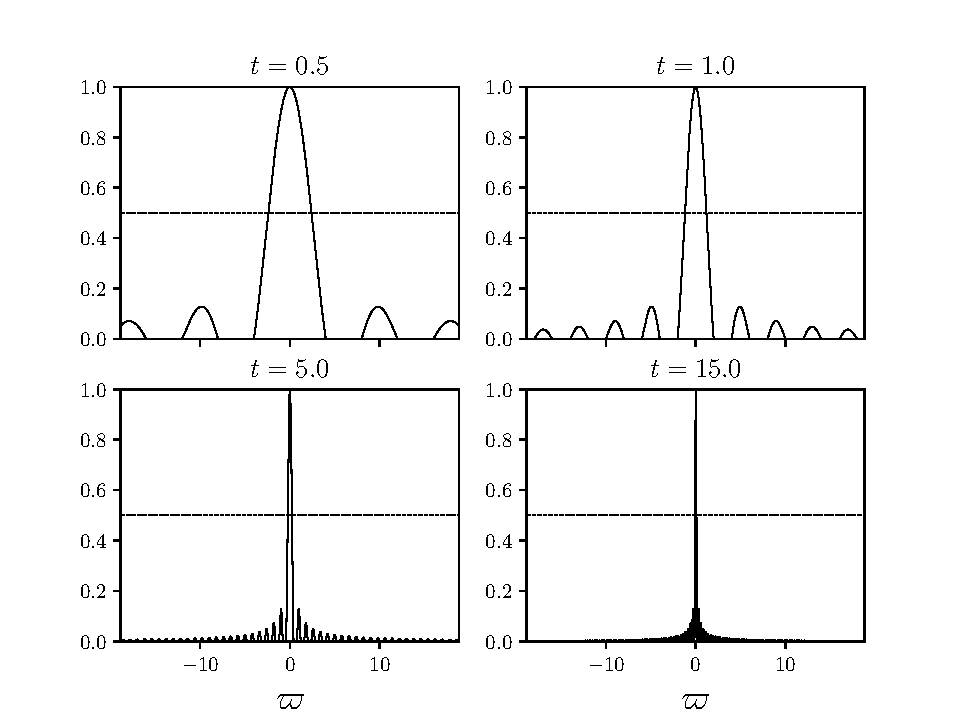
\includegraphics[scale=1]{Appendix-A/Figures/sinc_squared_plots.pdf}
 \caption[Plot of sinc-squared functions from quantum perturbation theory]{Plot of $\sinc^2 \left( \varpi t /2 \right)$ with $\varpi \equiv \left( \Delta \mathcal{E}_e - \Delta \gamma \right) / \hbar$ for four values of time $t$ using arbitrary units. Dashed lines mark half maximum of the central peak.}\label{fig:sinc_squared} %show that the central-peak width decreases with increasing $t$.
 \end{figure}
This is shown graphically in \cref{fig:sinc_squared}, where it is seen that the spectrum of possible photon energies for a first-order transition becomes narrower as time increases.\footnote{Note, however, that the factor of $t^2$ in \cref{eq:general_evolution5} is left out for the sake of comparison.} 

Depending on $\underline{\mathcal{H}}^{(\text{pert})}$, the quantity $\varpi = \left( \Delta \mathcal{E}_e - \Delta \gamma \right) / \hbar$ reduces to different forms. 
Processes that involve an electronic transition with a net change in binding energies, and either the absorption or emission of a single photon, can be described using first-order perturbations of the operator $\underline{\mathcal{H}}^{(1)} = (q_e / m_e) \, \underline{\mathbold{A}} ( \mathbold{r} ) \cdot \underline{\mathbold{p}}$ \cite[\emph{cf.\@} \cref{sec:ions_EM}]{Townsend00,Shankar04,Fontana_82,kapitell4,wysin2011quantization}. 
This can be seen by noting that $\underline{\mathcal{H}}^{(1)}$ depends linearly on both the Hilbert-space momentum operator $\underline{\mathbold{p}}$ and the Fock-space operators $\underline{a}_{\mathbold{k},\upsilon}$ and $\underline{a}^{\dagger}_{\mathbold{k},\upsilon}$ that are contained within the operator $\underline{\mathbold{A}} ( \mathbold{r} )$: 
\begin{align}\label{eq:single_photon_Hamiltonian}
 \begin{split}
 \underline{\mathcal{H}}^{(1)} = \frac{q_e}{m_e} \underline{\mathbold{A}} ( \mathbold{r} ) \cdot \underline{\mathbold{p}} &= \underbrace{\frac{q_e}{m_e} \sum_{\mathbold{k}} \sum_{\upsilon = 1}^2  \sqrt{\frac{\hbar}{2 \mathcal{V} \epsilon_0 \omega_{\mathbold{k}}}} \left( \hat{\mathbold{e}}_{\mathbold{k},\upsilon} \cdot \underline{\mathbold{p}} \right) \, \underline{a}_{\mathbold{k},\upsilon} \mathrm{e}^{i \mathbold{k} \cdot \mathbold{r} }}_{\text{absorption}} \\
 &+  \underbrace{\frac{q_e}{m_e} \sum_{\mathbold{k}} \sum_{\upsilon = 1}^2  \sqrt{\frac{\hbar}{2 \mathcal{V} \epsilon_0 \omega_{\mathbold{k}}}} \left( \hat{\mathbold{e}}_{\mathbold{k},\upsilon} \cdot \underline{\mathbold{p}} \right) \, \underline{a}^{\dagger}_{\mathbold{k},\upsilon} \mathrm{e}^{-i \mathbold{k} \cdot \mathbold{r}}}_{\text{emission}} . 
 \end{split}
 \end{align} 
In this case, $\varpi \to \left(\Delta \mathcal{E}_e - \hbar \omega_{\mathbold{k}} \right) / \hbar$ with $\mathcal{E}_B \neq \mathcal{E}_A$ and a photon number change of $\abs{N_{\mathbold{k}',\upsilon'}' - N_{\mathbold{k},\upsilon}} = 1$ [\emph{cf.\@} \cref{sec:single_absorption_emission}]. 
Therefore, the distribution in \cref{fig:sinc_squared} is a function of the absorbed or emitted photon energy with a centroid at $\Delta \mathcal{E}_e \equiv \hbar \omega_{\text{trans}}$, where $\omega_{\text{trans}}$ is the \emph{transition frequency}. 
On the other hand, $\underline{\mathcal{H}}^{(2)} = \left( q_e^2 / 2 m_e \right) \underline{\mathbold{A}}^2 \left( \mathbold{r} \right)$ contains cross-terms of the annihilation and creation operators: 
\begin{align}\label{eq:two_photon_Hamiltonian}
 \begin{split}
 &\underline{\mathcal{H}}^{(2)} = \frac{q_e^2}{2 m_e} \underline{\mathbold{A}}^2 \left( \mathbold{r} \right) \\
 &= \sum_{\mathbold{k},\mathbold{k}'} \sum_{\upsilon,\upsilon' = 1}^2 \left( \frac{\hbar q_e^2 \hat{\mathbold{e}}_{\mathbold{k},\upsilon} \cdot \hat{\mathbold{e}}_{\mathbold{k}',\upsilon'} }{4 \mathcal{V} \epsilon_0 m_e \omega_{\mathbold{k}} \, \omega_{\mathbold{k}'}} \right) \left[ \underline{a}_{\mathbold{k},\upsilon} \mathrm{e}^{i \mathbold{k} \cdot \mathbold{r} } + \underline{a}^{\dagger}_{\mathbold{k},\upsilon} \mathrm{e}^{-i \mathbold{k} \cdot \mathbold{r} } \right] \left[ \underline{a}_{\mathbold{k}',\upsilon'} \mathrm{e}^{i \mathbold{k}' \cdot \mathbold{r} } + \underline{a}^{\dagger}_{\mathbold{k}',\upsilon'} \mathrm{e}^{-i \mathbold{k}' \cdot \mathbold{r} } \right] 
 \end{split}
 \end{align} 
and so describes, among other two-photon processes, scattering phenomena, where $\underline{a}_{\mathbold{k},\upsilon}$ annihilates the initial photon and $\underline{a}^{\dagger}_{\mathbold{k}',\upsilon'}$ creates the scattered photon. 
In such a \emph{coherent scattering} process [\emph{cf.\@} \cref{sec:SXR_med}], the initial and final electron states are the same ($\mathcal{E}_B = \mathcal{E}_A$) while there is no change in the number of photons $\left( N_{\mathbold{k}',\upsilon'}' = N_{\mathbold{k},\upsilon} \right)$. 
As a result, the distribution in \cref{fig:sinc_squared} is in this case a function of scattered photon energy with a peak corresponding to the energy of the incident photon and $\varpi \to \omega_{\mathbold{k}'} - \omega_{\mathbold{k}}$.  

The first-order behavior just described is somewhat analogous to the spectrum of a finite, undamped sinusoidal wave in classical electrodynamics. 
To demonstrate this, let the following scalar function represent the strength of the electric field in such a wave as it passes by some fixed position over some duration, $\mathcal{T}$ \cite{Fontana82}:
\begin{subequations}
\begin{equation}\label{eq:wave}
    u(t) =
    \begin{cases}
      u_0 \cos \left( \Phi - \omega_0 t \right) , & 0 \leq t \leq \mathcal{T} \\
      0, & \text{otherwise.} 
    \end{cases}
  \end{equation}
The temporal Fourier transform of this function is 
\begin{align}
 \begin{split}
 u (\omega) &= \int_{-\infty}^{\infty} u(t) \, \mathrm{e}^{i \omega t} \dd{t} = u_0 \int_0^{\mathcal{T}} \cos \left( \Phi - \omega_0 t \right) \mathrm{e}^{i \omega t} \dd{t} \\
 &= \frac{i u_0}{2} \left( \mathrm{e}^{-i \Phi} \frac{1 - \mathrm{e}^{i \left( \omega + \omega_0 \right) \mathcal{T}}}{\left( \omega + \omega_0 \right)} + \mathrm{e}^{i \Phi} \frac{1 - \mathrm{e}^{i \left( \omega - \omega_0 \right) \mathcal{T}}}{\left( \omega - \omega_0 \right)} \right) ,
 \end{split}
 \end{align}
which describes two distributions in the frequency domain centered around $\omega = \pm \omega_0$ with full width at half maximum roughly equal to $2 \pi / \mathcal{T}$. 
Assuming that $\mathcal{T} \gg \omega_0^{-1}$, the contribution from the $\omega + \omega_0$ term can be neglected and then $\norm{u (\omega)}^2$, which is proportional to the energy density of the field, is \cite{Fontana82} 
\begin{equation}
 \norm{u (\omega)}^2 = \frac{u_0^2 \mathcal{T}^2}{4} \sinc^2 \left( \frac{\Delta \omega \mathcal{T}}{2} \right) ,
 \end{equation}
\end{subequations}
where $\Delta \omega \equiv \omega - \omega_0$.
Here, the parameter $\varpi \equiv \left( \Delta \mathcal{E}_e - \Delta \gamma \right) / \hbar$ used in this subsection is analogous to $\Delta \omega$ for a classical wave, where in \cref{fig:sinc_squared}, the spread of $\omega$ would become increasingly narrower as $\mathcal{T} \to \infty$. 

\subsection{Single-Photon Absorption and Emission}\label{sec:single_absorption_emission} 
%%%%%%%%%%%%%%%%%%%%%%%%%%%%%%%%%%%%%%--------------------------------------------------
Depending on the initial and final electron states, first-order perturbations of $\underline{\mathcal{H}}^{(1)}$ can describe bound-bound as well as bound-free absorption and emission processes. 
First, \emph{photo-absorption} can be described as a bound-bound state transition between an electron-photon states $\ket{A} = \ket{\Psi_G} \otimes \ket{N_{\mathbold{k},\upsilon}}$ and $\ket{B} = \ket{\Psi_E} \otimes \ket{\left( N_{\mathbold{k},\upsilon} - 1 \right)}$, where in the latter there is one photon missing from the original $N_{\mathbold{k},\upsilon}$ photons that are assumed to exist in a mode described by $\mathbold{k}$ and $\upsilon$ \cite{Townsend00}. 
Here, the transition is considered to take place in a hypothetical two-level atom with a ground state $\ket{\Psi_G}$ and an excited state $\ket{\Psi_E}$, with binding energies $\mathcal{E}_G$ and $\mathcal{E}_E$ (assuming $\mathcal{E}_E > \mathcal{E}_G$).
In the context of astrophysical soft x-ray spectroscopy, this can be taken to represent one mode of the x-ray continuum source generated by an active galactic nucleus that is absorbed by a particular transition in a highly-charged ion [\emph{cf.\@} \cref{sec:astro_plasmas}]. 
The probability for absorption to occur as a function of time according to \cref{eq:prob_matrix_element} is \cite{Shankar04,Townsend00,kapitell4,wysin2011quantization} 
\begin{align}\label{eq:absorption_evolution4}
 \begin{split}
 &\mathscr{P}_{G \to E} (t) \equiv \norm{\bra{\Psi_E} \otimes \bra{\left( N_{\mathbold{k},\upsilon} -1 \right)} \underline{U}_I (t) \ket{\Psi_G} \otimes \ket{N_{\mathbold{k},\upsilon}}}^2 \\
 &= \frac{t^2}{\hbar^2} \norm{\mathcal{M}_{\text{abso}}}^2 \sinc^2 \left( \frac{\varpi t}{2} \right) \quad \text{where } \varpi \equiv \omega_{\text{trans}} - \omega_{\mathbold{k}} .
 \end{split}
 \end{align}
With $\underline{\mathcal{H}}^{(1)} = \left( q_e / m_e \right) \underline{\mathbold{A}} ( \mathbold{r} ) \cdot \underline{\mathbold{p}}$ given by \cref{eq:single_photon_Hamiltonian} as the perturbing operator, $\norm{\mathcal{M}_{\text{abso}}}^2$ can be evaluated by carrying out the following Fock-space operations: 
\begin{align} 
\begin{split}\label{eq:Fock_operations}
 &\bra{\Psi_E} \otimes \bra{\left( N_{\mathbold{k},\upsilon} -1 \right)} \underline{\mathbold{A}} ( \mathbold{r} ) \cdot \underline{\mathbold{p}} \ket{\Psi_G} \otimes \ket{N_{\mathbold{k},\upsilon}} \\
 &\: = \bra{\Psi_E} \otimes \bra{\left( N_{\mathbold{k},\upsilon} -1 \right)} \sum_{\mathbold{k}'} \sum_{\upsilon' = 1}^2 \sqrt{\frac{\hbar}{2 \mathcal{V} \epsilon_0 \omega_{\mathbold{k}'}}} \left( \hat{\mathbold{e}}_{\mathbold{k}',\upsilon'} \cdot \underline{\mathbold{p}} \right) \underline{a}_{\mathbold{k}',\upsilon'} \mathrm{e}^{i \mathbold{k}' \cdot \mathbold{r} } \ket{\Psi_G} \otimes \ket{N_{\mathbold{k},\upsilon}} \\
 &\; + \bra{\Psi_E} \otimes \bra{\left( N_{\mathbold{k},\upsilon} -1 \right)} \sum_{\mathbold{k}'} \sum_{\upsilon' = 1}^2 \sqrt{\frac{\hbar}{2 \mathcal{V} \epsilon_0 \omega_{\mathbold{k}'}}} \left( \hat{\mathbold{e}}_{\mathbold{k}',\upsilon'} \cdot \underline{\mathbold{p}} \right) \underline{a}^{\dagger}_{\mathbold{k}',\upsilon'} \mathrm{e}^{-i \mathbold{k}' \cdot \mathbold{r} } \ket{\Psi_G} \otimes \ket{N_{\mathbold{k},\upsilon}} \\
 &\: = \sqrt{\frac{\hbar N_{\mathbold{k},\upsilon}}{2 \mathcal{V} \epsilon_0 \omega_{\mathbold{k}}}} \hat{\mathbold{e}}_{\mathbold{k},\upsilon} \cdot \bra{\Psi_B} \underline{\mathbold{p}} \mathrm{e}^{i \mathbold{k} \cdot \mathbold{r} } \ket{\Psi_G} \underbrace{\braket{\left( N_{\mathbold{k},\upsilon} - 1 \right)}}_{1} \\
 &\; + \sqrt{\frac{\hbar \left( N_{\mathbold{k},\upsilon} + 1 \right)}{2 \mathcal{V} \epsilon_0 \omega_{\mathbold{k}}}} \hat{\mathbold{e}}_{\mathbold{k},\upsilon} \cdot \bra{\Psi_E} \underline{\mathbold{p}} \mathrm{e}^{-i \mathbold{k} \cdot \mathbold{r} } \ket{\Psi_G} \underbrace{\braket{\left( N_{\mathbold{k},\upsilon} - 1 \right)}{\left( N_{\mathbold{k},\upsilon} + 1 \right)}}_{0}
 \end{split}
 \end{align}
so that it becomes\footnote{The evaluation of $\hat{\mathbold{e}}_{\mathbold{k},\upsilon} \cdot \bra{\Psi_E} \underline{\mathbold{p}} \mathrm{e}^{ i \mathbold{k} \cdot \mathbold{r}} \ket{\Psi_G}$ is handled in \cref{ap:quantum_spectral}. }
\begin{align}
 \begin{split}
 \norm{\mathcal{M}_{\text{abso}}}^2 &= \norm{\bra{\Psi_E} \otimes \bra{\left( N_{\mathbold{k},\upsilon} -1 \right)} \underline{\mathcal{H}}^{(1)} \ket{\Psi_G} \otimes \ket{N_{\mathbold{k},\upsilon}}}^2 \\ 
 &= \frac{q_e^2}{m_e^2} \norm{\bra{\Psi_E} \otimes \bra{\left( N_{\mathbold{k},\upsilon} -1 \right)} \underline{\mathbold{A}} ( \mathbold{r} ) \cdot \underline{\mathbold{p}} \ket{\Psi_G} \otimes \ket{N_{\mathbold{k},\upsilon}}}^2 \\
 &= \frac{q_e^2 \hbar N_{\mathbold{k},\upsilon}}{2 m_e^2 \mathcal{V} \epsilon_0 \omega_{\mathbold{k}}} \norm{\hat{\mathbold{e}}_{\mathbold{k},\upsilon} \cdot \bra{\Psi_E} \underline{\mathbold{p}} \mathrm{e}^{ i \mathbold{k} \cdot \mathbold{r}} \ket{\Psi_G}}^2 ,
 \end{split}
 \end{align}
Single-photon absorption can also occur as a bound-free process known as \emph{photo-ionization}, or the \emph{photo-electric effect}, where a photon with $\mathcal{E}_{\gamma}$ just exceeding $\mathcal{E}_e$ is absorbed as the electron is ejected with kinetic energy equal to $\mathcal{E}_{\gamma} - \mathcal{E}_e$ \cite{Kahn02}.\footnote{\emph{e.g.}, from a highly-charged ion in a cosmic plasma or a neutral atom in a material} 
In this case, the initial state is taken to be the ground state with $\ket{A} = \ket{\Psi_G} \otimes \ket{N_{\mathbold{k},\upsilon}}$ but the final state is $\ket{B} = \ket{\Psi_C} \otimes \ket{\left( N_{\mathbold{k},\upsilon} - 1 \right)}$, where $\ket{\Psi_C}$ is a continuum state for a free electron. 
This phenomenon can occur in cosmic plasmas with a strong soft x-ray field as well as in materials where \emph{absorption edges} are formed [\emph{cf.\@} \cref{sec:SXR_med}]. 

Conversely, bound-bound \emph{stimulated emission} can be described as being precisely the opposite of the photo-absorption process where there is an electron-photon state change from $\ket{A} = \ket{\Psi_E} \otimes \ket{\left( N_{\mathbold{k},\upsilon} -1 \right)}$ to $\ket{B} = \ket{\Psi_G} \otimes \ket{N_{\mathbold{k},\upsilon}}$. 
Their matrix elements are therefore complex conjugates of one another:
\begin{equation}
\bra{\Psi_G} \otimes \bra{N_{\mathbold{k},\upsilon}} \underline{U}_I (t) \ket{\Psi_E} \otimes \ket{\left( N_{\mathbold{k},\upsilon} -1 \right)} = \bra{\Psi_E} \otimes \bra{\left( N_{\mathbold{k},\upsilon} -1 \right)} \underline{U}_I (t) \ket{\Psi_G} \otimes \ket{N_{\mathbold{k},\upsilon}}^* 
 \end{equation}
so that from the Fock-state operations of \cref{eq:Fock_operations}, it follows that
\begin{align}\label{eq:abso_stim_balance}
 \begin{split}
 \mathcal{M}_{\text{stim}} &\equiv \bra{\Psi_G} \otimes \bra{N_{\mathbold{k},\upsilon}} \underline{\mathcal{H}}^{(1)} \ket{\Psi_E} \otimes \ket{\left( N_{\mathbold{k},\upsilon} - 1 \right)} = \mathcal{M}_{\text{abso}}^* \\
 &= \hat{\mathbold{e}}_{\mathbold{k},\upsilon} \cdot \bra{\Psi_G} \underline{\mathbold{p}} \mathrm{e}^{ -i \mathbold{k} \cdot \mathbold{r}} \ket{\Psi_E}
 \end{split}
 \end{align}
and as a result, $\norm{\mathcal{M}_{\text{abso}}}^2 = \norm{\mathcal{M}_{\text{stim}}}^2$. 
This implies that for either photo-absorption or stimulated emission, the probability as a function of time for any transition between two electron-photon states $\ket{A}$ and $\ket{B}$ is of the form given by \cref{eq:general_evolution5}, where assuming that the photon changes from $\ket{N_{\mathbold{k},\upsilon}}$ to $\ket{\left( N_{\mathbold{k},\upsilon} - 1 \right)}$ or vice-versa, $\mathcal{M}$ is either $\mathcal{M}_{\text{abso}}$ or $\mathcal{M}_{\text{stim}}$. 
In either case, after all Fock-state operations have been carried out, the norm squared of this matrix element is 
\begin{equation}\label{eq:abso_stim_matrix_element}
 \norm{\mathcal{M}}^2 = \frac{q_e^2 \hbar N_{\mathbold{k},\upsilon}}{2 m_e^2 \mathcal{V} \epsilon_0 \omega_{\mathbold{k}}} \norm{\hat{\mathbold{e}}_{\mathbold{k},\upsilon} \cdot \bra{\Psi_B} \underline{\mathbold{p}} \mathrm{e}^{\pm i \mathbold{k} \cdot \mathbold{r}} \ket{\Psi_A}}^2 ,
 \end{equation}
where in the complex exponential, the $+$ and $-$ signs correspond to emission and absorption, respectively. 
This demonstrates that, in addition to the effect that $\underline{\mathbold{p}} \mathrm{e}^{\pm i \mathbold{k} \cdot \mathbold{r}}$ has as a perturbing operator, the probability of a photon with energy $\mathcal{E}_{\gamma} = \hbar \omega_{\mathbold{k}}$ being absorbed depends on $N_{\mathbold{k},\upsilon}$, the number of photons present in a particular mode defined by $\mathbold{k}$ and $\upsilon$. 
Moreover, \emph{radiative recombination} can occur as a free-bound process, where a free electron (\emph{e.g.}, one in a cosmic plasma) with speed $v_e$ and kinetic energy $\frac{1}{2} m_e v_e^2$ fills a vacancy in an ion with a binding energy $\mathcal{E}_e$ and a photon of energy $\frac{1}{2} m_e v_e^2 - \mathcal{E}_e$ is emitted in the process. 
This process can be thought of as the opposite of photo-ionization, where an electron is absorbed by an ion as a photon is emitted. 
Taking the vacancy to be filled as the ground state, this can be described as a change in state from $\ket{A} = \ket{\Psi_C} \otimes \ket{N_{\mathbold{k},\upsilon}}$ (where $\ket{\Psi_C}$ is a continuum state) to $\ket{B} = \ket{\Psi_G} \otimes \ket{\left( N_{\mathbold{k},\upsilon} + 1 \right)}$. 

Both photo-absorption and stimulated emission can also be understood as arising from the presence of a classical electromagnetic wave, where the classical vector potential $\mathbold{A} ( \mathbold{r} , t)$ [\emph{cf.\@} \cref{eq:potential_wave_solution}] is used in place of the vector potential operator $\underline{\mathbold{A}} ( \mathbold{r} )$ \cite[\emph{cf.\@} \cref{eq:vector_potential_operator_fixedtime}]{Rybicki86,Shankar04}. 
Although this is justified for large photon numbers, where the radiation can be treated as a coherent state [\emph{cf.\@} \cref{sec:coherent_states}], the classical-wave approximation does not necessarily hold in x-ray astrophysics, where photon counts typically are low. 
%As discussed in \cref{sec:coherent_states}, this is justified for large photon numbers where the radiation can be treated as a coherent state. 
%However, in x-ray astrophysics where photon counts are low, the classical-wave approximation does not necessarily hold 
Moreover, a photon description of radiation is needed to explain the phenomenon of \emph{spontaneous emission}, where there is no stimulating radiation field. 
This process can be described as a transition from $\ket{A} = \ket{\Psi_E} \otimes \ket{0}$ to $\ket{B} = \ket{\Psi_G} \otimes \ket{1_{\mathbold{k},\upsilon}}$, where a photon is emitted from the vacuum state \cite{Fontana_82,Townsend00,Shankar04}. 
In this case, \cref{eq:abso_stim_matrix_element} holds with $N_{\mathbold{k},\upsilon} = 1$ so that the matrix element is
\begin{align}\label{eq:emission_matrix_element}
 \begin{split}
 \mathcal{M}_{\text{spon}} &\equiv \bra{\Psi_G} \otimes \bra{1_{\mathbold{k},\upsilon}} \underline{\mathcal{H}}^{(1)} \ket{\Psi_E} \otimes \ket{0} \\
 &= \frac{q_e}{m_e} \sqrt{\frac{\hbar}{2 \mathcal{V} \epsilon_0 \omega_{\mathbold{k}}}} \hat{\mathbold{e}}_{\mathbold{k},\upsilon} \cdot \bra{\Psi_G} \underline{\mathbold{p}} \mathrm{e}^{-i \mathbold{k} \cdot \mathbold{r}} \ket{\Psi_E}  .
 \end{split}
 \end{align}
This is often the prominent mechanism for discrete photon emission in diffuse plasmas where the soft x-ray field is too weak to induce stimulated emission appreciably. 
Two-photon processes, including second-order perturbations of $\underline{\mathcal{H}}^{(1)}$ as well as first-order perturbations of $\underline{\mathcal{H}}^{(2)}$, can also occur in bound-bound transitions.\footnote{\emph{e.g.}, in helium-like ions as described in \cref{sec:selection_rules_helium}} 
However, since the probability for a transition to occur depends on the norm squared of a matrix element involving $\underline{\mathcal{H}}^{(\text{pert})}_I (t)$, single-photon processes are proportional to the fine-structure constant, $\alpha_f \equiv q^2_e / 4 \pi \epsilon_0 \hbar c_0$, while two-photon process are proportional to $\alpha_f^2$ [\emph{cf.\@} \cref{eq:coupled_Hamiltonian3}]. 
Because of this, transitions associated with first-order $\underline{\mathcal{H}}^{(1)}$ are significantly more likely to occur than those associated with first-order $\underline{\mathcal{H}}^{(2)}$ or second-order $\underline{\mathcal{H}}^{(1)}$ \cite{Shankar04,Townsend00}. 
For this reason, single-photon transitions are what contribute the most to soft x-ray spectra from the hot, diffuse plasmas described in \cref{sec:astro_plasmas}, where scattering can also typically be neglected \cite{Paerels03}. 

\subsection{Transition Rates}\label{sec:transition_rate_sub}
%%%%%%%%%%%%%%%%%%%%%%%%%%%%%%%%%%%%%%%%%--------------------------------------------------
The $t \to \infty$ first-order behavior described by \cref{eq:general_evolution5} can be used to derive a typical transition rate for a given process characterized by a time-independent matrix element, $\mathcal{M}$. 
Using $\Delta \mathcal{E}_e$ and $\Delta \gamma \equiv N_{\mathbold{k}',\upsilon'}' \, \hbar \omega_{\mathbold{k}'} - N_{\mathbold{k},\upsilon} \, \hbar \omega_{\mathbold{k}}$ introduced in \cref{sec:gen_first_order}, this transition rate can be determined from the following expression:
\begin{subequations}
\begin{equation}\label{eq:trans_rate_sigle_mode_general}
 \frac{\mathscr{P}_{A \to B}^{\infty} (t)}{t} = \frac{2 \pi}{\hbar} \norm{\mathcal{M}}^2 \delta_D \left( \Delta \mathcal{E}_e - \Delta \gamma \right) , 
 \end{equation}
which is independent of time. 
While this approach can be used to calculate transition rates for any first-order process, the main interest here is to determine the relative transition rates of various bound-bound transitions in highly-charged ions as addressed in \cref{ap:quantum_spectral}. 
In this case, \cref{eq:trans_rate_sigle_mode_general} with $\Delta \gamma = \hbar \omega_{\mathbold{k}}$ becomes 
\begin{equation}\label{eq:trans_rate_sigle_mode}
 \Gamma_{\upsilon} (\hbar \omega_{\mathbold{k}}) \equiv  \frac{\mathscr{P}_{A \to B}^{\infty} (t)}{t} = \frac{2 \pi}{\hbar} \norm{\mathcal{M}}^2 \delta_D \left( \Delta \mathcal{E}_e - \hbar \omega_{\mathbold{k}} \right) , 
 \end{equation}
\end{subequations}
a time-independent function of $\mathcal{E}_{\gamma} = \hbar \omega_{\mathbold{k}}$. 
However, a realistic spectral line is formed from a large number of ions undergoing the same process with probabilistic values for $\mathcal{E}_{\gamma}$ and photon-propagation direction, $\mathbold{k} / k_0$. 

To take into account a range of $\mathcal{E}_{\gamma}$ and $\mathbold{k} / k_0$, recall that the electromagnetic field has been quantized using boundary conditions imposed by a large box of volume $\mathcal{V}$ [\emph{cf.\@} \cref{sec:photon_intro}]. 
This means that, mathematically, the possible photon modes are restricted to a lattice where there are a finite number of these states with wave vector between $\mathbold{k}$ and $\mathbold{k}+ \mathbold{\Delta k}$ to consider. 
Following Townsend~\cite{Townsend00}, the number of modes with wave number in between $k_0$ and $k_0 + \Delta k_0$, and propagation-direction solid angle between $\Omega$ and $\Omega + \Delta \Omega$, can be written as  
\begin{subequations}
\begin{equation}\label{eq:photon_states1}
 \frac{\mathcal{V}}{\left( 2 \pi \right)^3} k_0^2 \Delta k_0 \Delta \Omega \to \frac{\mathcal{V}}{\left( 2 \pi \right)^3} k_0^2 \dd{k_0} \dd{\Omega} , 
 \end{equation}
where infinitesimal intervals are used in the limit that $\mathcal{V} \to \infty$ to describe a physical system. 
In terms of photon energy, this is written as
\begin{equation}\label{eq:photon_states2}
 \frac{\mathcal{V}}{\left( 2 \pi \right)^3} k_0^2 \dd{k_0} \dd{\Omega} = \frac{\mathcal{V}}{\left( h c_0 \right)^3} \mathcal{E}^2_{\gamma} \dd{\mathcal{E}_{\gamma}} \dd{\Omega} \equiv \rho_{\text{state}} \left( \mathcal{E}_{\gamma} \right) \dd{\mathcal{E}_{\gamma}} \dd{\Omega} , 
 \end{equation}
where
\begin{equation}\label{eq:photon_state_density}
 \rho_{\text{state}} \left( \mathcal{E}_{\gamma} \right) \equiv  \frac{\mathcal{V}}{\left( h c_0 \right)^3} \mathcal{E}^2_{\gamma} \quad \text{or} \quad \rho_{\text{state}} \left( \omega_{\mathbold{k}} \right) \equiv \frac{\mathcal{V}}{\left( 2 \pi \right)^3} \frac{\omega_{\mathbold{k}}^2}{\hbar c_0^3}
 \end{equation}
is the \emph{density of photon states} per photon energy, per solid angle \cite{Townsend00}.  
\end{subequations}

With the transition probability for a single photon mode being $\norm{\bra{B} \underline{U}_I (t) \ket{A}}^2$, the overall transition probability taking into account the range of photon modes is calculated from summing $\norm{\bra{B} \underline{U}_I (t) \ket{A}}^2$ over all possible states. 
In the limit that $\mathcal{V} \to \infty$, the summation of these probabilities for a single polarization mode becomes an integral using \cref{eq:photon_states1,eq:photon_states2,eq:photon_state_density}:
\begin{align}\label{eq:absorption_evolution6}
 \begin{split}
 \mathscr{P}_{\upsilon} (t) \equiv \sum_{\mathbold{k}}^{\mathbold{k} + \mathbold{\Delta k}} \norm{\bra{B} \underline{U}_I (t) \ket{A}}^2 &\to \frac{\mathcal{V}}{\left( 2 \pi \right)^3} \int k_0^2 \dd{k_0} \int \dd{\Omega} \norm{\bra{B} \underline{U}_I (t) \ket{B}}^2 \\
 &= \int \rho_{\text{state}} \left( \mathcal{E}_{\gamma} \right) \dd{\mathcal{E}_{\gamma}} \int \dd{\Omega} \norm{\bra{B} \underline{U}_I (t) \ket{A}}^2 
 \end{split}
 \end{align}
and from \cref{eq:trans_rate_sigle_mode}, it is known that 
\begin{equation*}
 \mathscr{P}_{A \to B}^{\infty} (t) \equiv \lim_{t \to \infty} \norm{\bra{B} \underline{U}_I (t) \ket{A}}^2 = \frac{2 \pi t}{\hbar} \norm{\mathcal{M}}^2 \delta_D \left( \Delta \mathcal{E}_e - \mathcal{E}_{\gamma} \right) = t \, \Gamma_{\upsilon} (\mathcal{E}_{\gamma}) .
 \end{equation*}
Therefore, using \cref{eq:absorption_evolution6}, the probability of the transition occurring in the long-time limit (for a single polarization mode) is 
\begin{align}
 \begin{split}\label{eq:long_time_trans_prob}
 \mathscr{P}_{\upsilon}^{\infty} &\equiv \lim_{t \to \infty} \mathscr{P}_{\upsilon} (t) = \frac{2 \pi t}{\hbar} \int \rho_{\text{state}} \left( \mathcal{E}_{\gamma} \right) \dd{\mathcal{E}_{\gamma}} \int \norm{\mathcal{M}}^2 \delta_D \left( \Delta \mathcal{E}_e - \mathcal{E}_{\gamma} \right) \dd{\Omega} \\
 &= \frac{2 \pi t}{\hbar} \int \rho_{\text{state}} \left( \Delta \mathcal{E}_e \right) \norm{\mathcal{M}}^2 \Big|_{\mathcal{E}_{\gamma} = \Delta \mathcal{E}_e} \dd{\Omega} = t \int \rho_{\text{state}} \left( \Delta \mathcal{E}_e \right) \Gamma_{\upsilon} (\Delta \mathcal{E}_e) \dd{\Omega} ,
 \end{split}
 \end{align}
where, along with $\rho_{\text{state}} \left( \mathcal{E}_{\gamma} \right)$, $\mathcal{M}$, and $\Gamma_{\upsilon} (\mathcal{E}_{\gamma})$ are evaluated at $\mathcal{E}_{\gamma} = \Delta \mathcal{E}_e$ \cite{Shankar04,Townsend00,Griffiths05}. 
While this is an approximation, $\mathscr{P}_{\upsilon}^{\infty}$ can be used to obtain a probabilistic rate for a certain transition. 
Per solid angle, for a single polarization state, this can be defined as 
\begin{subequations}
\begin{align}
 \begin{split}\label{eq:diff_transition_rate}
 \Gamma_{\upsilon \Omega} \equiv \dv{\Omega}(\frac{\mathscr{P}_{\upsilon}^{\infty}}{t}) &= \frac{2 \pi}{\hbar} \rho_{\text{state}} \left( \Delta \mathcal{E}_e \right) \norm{\mathcal{M}}^2 \Big|_{\mathcal{E}_{\gamma} = \Delta \mathcal{E}_e} \\
 &= \frac{\mathcal{V}}{4 \pi^2 \hbar^2 c_0^3} \left( \frac{\Delta \mathcal{E}_e}{\hbar} \right)^2  \norm{\mathcal{M}}^2 \Big|_{\mathcal{E}_{\gamma} = \Delta \mathcal{E}_e} \propto \omega_{\text{trans}}^2 ,
 \end{split}
 \end{align}
while the total transition rate is obtained from summing over both polarization states and integrating over the solid angle of interest:
\begin{equation}\label{eq:transition_rate}
 \Gamma \equiv \sum_{\upsilon = 1}^2 \int \Gamma_{\upsilon \Omega} \dd{\Omega} .
 \end{equation}
\end{subequations}
The idea that the probability rate for a given transition is approximately independent of time according to \cref{eq:diff_transition_rate,eq:transition_rate} is known as \emph{Fermi's golden rule} \cite{Townsend00,Kahn02,Shankar04,kapitell4,wysin2011quantization}. 
The fact that $\Gamma_{\upsilon \Omega} \propto \omega_{\text{trans}}^2$ implies that transition rates for processes involving soft x-rays are expected to be large compared to those associated with lower-energy radiation due to their relatively high photon energy. % $\mathcal{E}_{\gamma} = \Delta \mathcal{E}_e$. 
An important consequence of this is that highly-charged ions undergoing soft x-ray transitions require high rates of excitation for local thermodynamic equilibrium to be established in a cosmic plasma \cite{Paerels03}. 

\section{Summary}\label{sec:apAsummary}
%%%%%%%%%%%%%%%%%%%%%%%%%%%%%%%%%%%%%%%%%--------------------------------------------------
This appendix outlines mathematical framework for discussions relating to soft x-ray interaction with matter throughout this dissertation. 
In particular, the classical description of electromagnetic waves laid out in \cref{sec:EM_waves_vac} is used as a starting point for x-ray optics discussion in \cref{ch:diff_eff,app:x-ray_materials}. 
Photons are described quantum-mechanically as vectors in Fock space that are acted upon by annihilation and creation operators contained within Hermitian operators for the electromagnetic field. 
Their interaction with atomic electrons, which are described quantum-mechanically as vectors in Hilbert space, is treated in \cref{sec:atomic_interaction} as a segue into \cref{ap:quantum_spectral}, which addresses spectral lines produced from highly-charged ions found in cosmic plasmas. 